\documentclass[preprint,12pt]{elsarticle}
\usepackage{lmodern}
\ifdefined\pdfgentounicode
\input{glyphtounicode}
\pdfgentounicode=1
\fi
\usepackage{amsmath,amssymb,amsfonts,mathtools,amsthm,bm}
\usepackage{booktabs,graphicx,array,tabularx,longtable,float,url}
\usepackage{needspace}
\usepackage{placeins}
\usepackage[hidelinks]{hyperref}
\hypersetup{pdfauthor={Ali Eslami and Jiangbo Yu}}
\usepackage[protrusion=true,expansion=false]{microtype}
\graphicspath{{figures/}{./}}
\allowdisplaybreaks
\setlength{\emergencystretch}{3em}
\interdisplaylinepenalty=2500
\theoremstyle{definition}
\newtheorem{assumption}{Assumption}
\theoremstyle{plain}
\newtheorem{theorem}{Theorem}
\newtheorem{proposition}{Proposition}
\newtheorem{lemma}{Lemma}
\newtheorem{corollary}{Corollary}
\newtheorem{remark}{Remark}
\theoremstyle{definition}
\newtheorem{definition}{Definition}
\newtheorem{problem}{Problem}
\theoremstyle{plain}
\floatstyle{ruled}
\newfloat{algorithm}{tbp}{loa}
\floatname{algorithm}{Algorithm}
\newcommand{\R}{\mathbb{R}}
% elsarticle includes the word ``Appendix'' in appendix-section references.
\newcommand{\appref}[1]{\ref{#1}}
\newcommand{\longpaperdetails}[1]{#1 of the \href{https://github.com/AlienEslami/agentic-perimeter-runtime-certification/blob/main/paper/main.pdf}{long version}}
\newcommand{\reproductiondetails}[1]{\href{https://github.com/AlienEslami/agentic-perimeter-runtime-certification/releases/tag/paper-2026-11-11}{#1}~\cite{perimeterReproductionGuide}}
\journal{Transportation Research Part B: Methodological}


% Reduced manuscript: certification structure and supporting appendices, 10 November 2026.
\begin{document}
\begin{frontmatter}
\title{A Formal Guarantee for Trustworthy Agentic Traffic Control: A Multi-region Perimeter Case}
\author[mcgill]{Ali Eslami}
\ead{ali.eslami@mcgill.ca}
\author[mcgill]{Jiangbo Yu\corref{cor1}}
\ead{jiangbo.yu@mcgill.ca}
\cortext[cor1]{Corresponding author.}
\affiliation[mcgill]{organization={Department of Civil Engineering, McGill University},
 addressline={817 Sherbrooke Street West}, city={Montreal}, state={Quebec},
 postcode={H3A 0G4}, country={Canada}}
\begin{abstract}\fontsize{11}{13}\selectfont
Perimeter control helps reduce urban congestion by regulating traffic flows
between regions. Control plans may need to be revised as traffic conditions
and operating priorities change. Artificial intelligence (AI) agents can
support this process by interpreting operator instructions and using tools
to develop control plans. However, each new agent-proposed plan must remain
compatible with the evolving traffic state, uncertainty, and outstanding
service requirements. In this paper, we develop a dual-agent framework in
which an AI agent proposes plans and a rule-based supervisory agent checks
them before execution. Using vehicle-conserving traffic dynamics, the supervisor checks
nonnegative traffic states, boundary-storage limits, and service deadlines
under bounded state-estimation and arrival-forecast errors. It determines whether the plan can be executed as
proposed, needs modification to meet these requirements, or should be
rejected while the current plan continues under its existing guarantee.
We also establish conditions for maintaining these guarantees beyond a
plan's specified duration. Numerical studies show that the framework can
accept plans unchanged and repair proposals to meet the requirements. Further
experiments show that the framework
can accept beneficial changes while rejecting requests that would violate
boundary-storage or service requirements, including under computation
delays and agent-context errors. Overall, the framework supports
trustworthy AI for transportation by connecting adaptive agent decisions
to traffic control while satisfying physical limits and service requirements.
\end{abstract}
\begin{keyword}
Urban perimeter control \sep Macroscopic fundamental diagram \sep Agentic AI \sep Formal guarantees
\end{keyword}
\end{frontmatter}


\section{Introduction}
\label{sec:new-introduction}

Traffic control coordinates vehicle movements to reduce delay and manage
congestion across an urban network. Intersection control allocates signal
time among competing movements, while coordinated control links decisions
across intersections and corridors. Network-level strategies account for
interactions across a wider area \cite{papageorgiou2003review}.
At the regional scale, urban perimeter
control regulates the flows between areas of the network and their
surroundings. Restricting entry to a congested region can
improve traffic conditions inside it, but may also cause queues to grow at
its boundary. Control decisions must therefore account for both regional
congestion and the storage capacity of boundary queues
\cite{haddad2017queues}. One approach to modeling regional traffic uses
the macroscopic fundamental diagram (MFD), which relates the number of
vehicles in a region to its aggregate outflow
\cite{geroliminis2008existence,daganzo2008analytical,geroliminis2011properties}.
Figure~\ref{fig:regional-traffic-overview} illustrates the regional traffic flows
and entry queues considered in this setting.

\begin{figure}[!t]
\centering
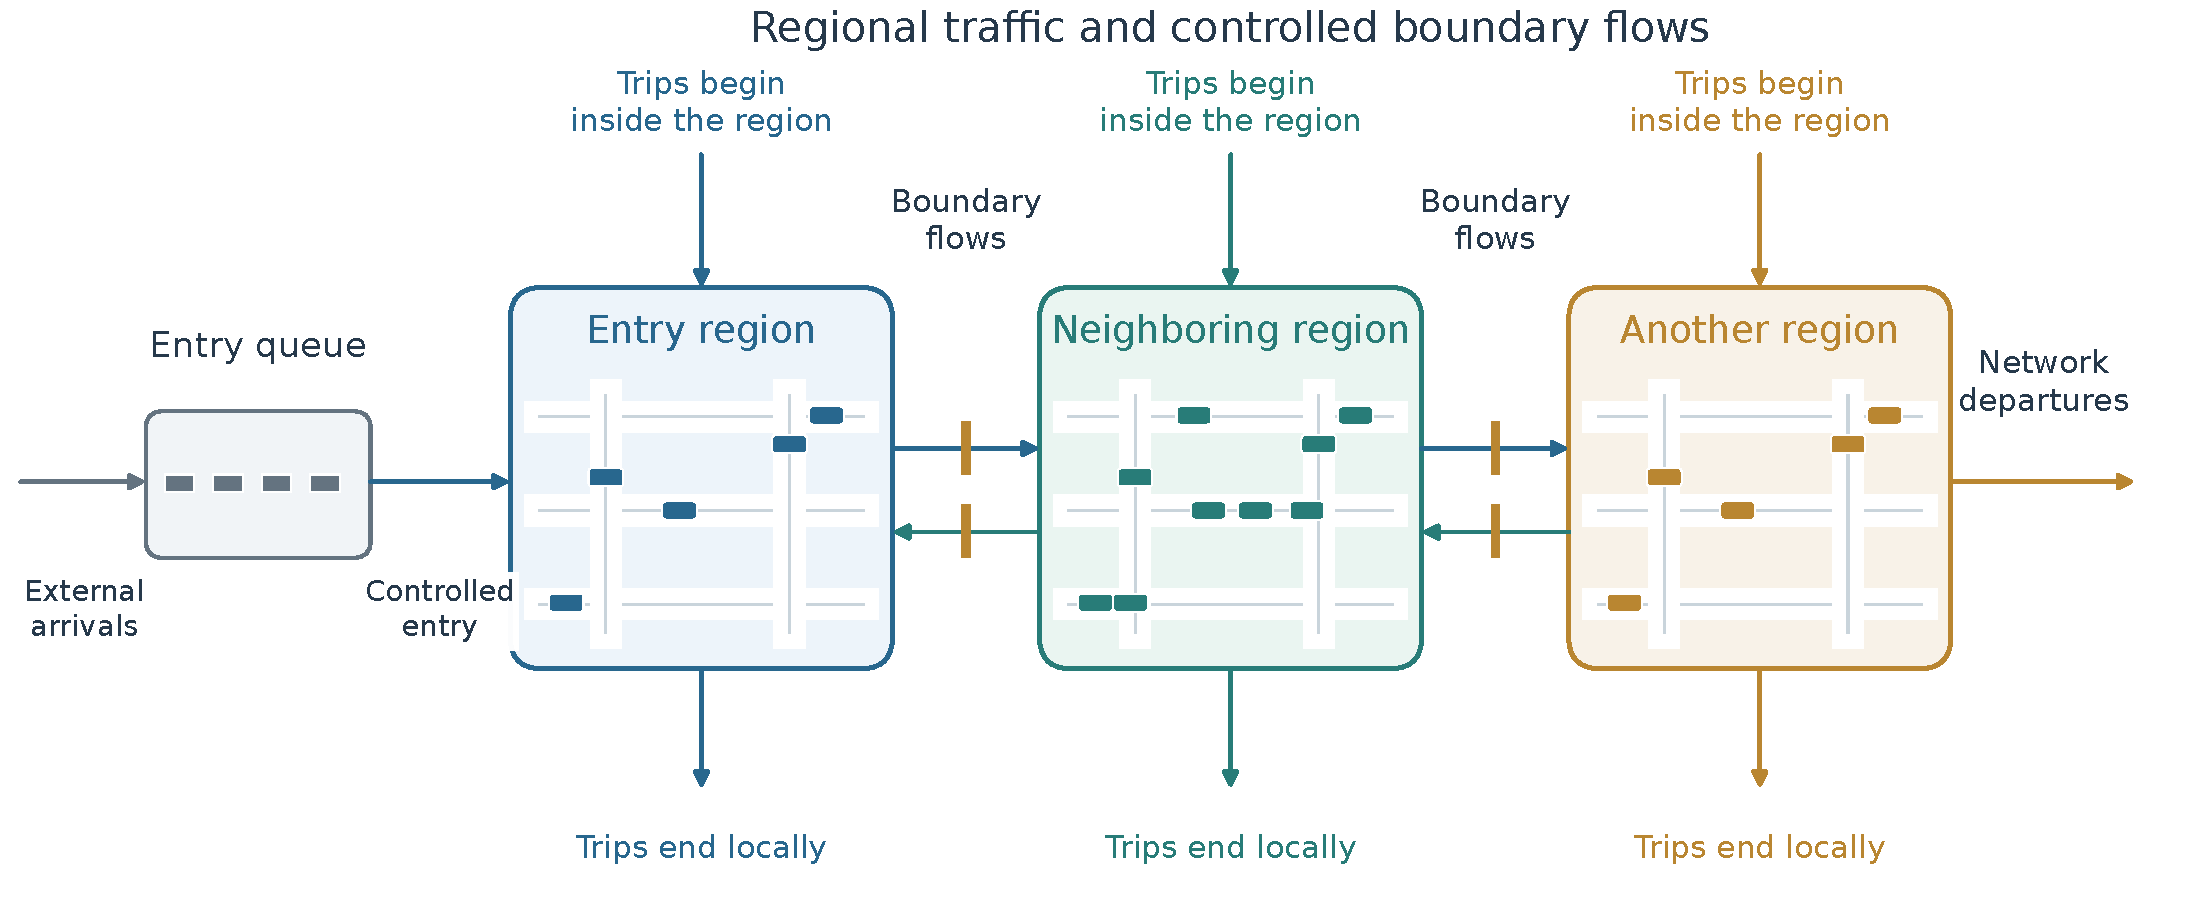
\includegraphics[width=\textwidth]{figures/regional_traffic_overview.pdf}
\caption{Regional perimeter control. Vehicles enter through boundary
queues, move between connected regions, complete trips within a region,
or leave the network. New trips also begin inside the regions. Perimeter
control regulates the boundary flows, while regional traffic conditions
determine how quickly vehicles move. The regions and roads are schematic,
and the number of regions and entry queues depends on the application.}
\label{fig:regional-traffic-overview}
\end{figure}

Within this modeling framework, feedback control methods adjust boundary
flows in response to observed traffic conditions
\cite{keyvan2012gating,aboudolas2013perimeter}. Predictive methods use the
traffic model and demand forecasts to select control actions over a
planning horizon \cite{geroliminis2013mpc,sirmatel2018economic}. Related
formulations explicitly account for boundary queues and their storage
limits \cite{haddad2017queues}. Robust control methods address uncertain
demand and limited traffic measurements, with stability and robustness
guarantees established under specified modeling assumptions
\cite{zhong2018robust,mohajerpoor2020hinf}. Earlier robust perimeter-control
formulations also address MFD uncertainty and uncertain destination
decomposition, including constrained interpolation-based control
\cite{haddad2014robust,haddad2015robust}.

Data-driven approaches have also been developed for perimeter control.
Reinforcement learning and adaptive dynamic programming use traffic
observations and the outcomes of control actions to learn control policies
\cite{chen2022dataefficient,chen2024iadp}. Multi-agent reinforcement
learning supports coordination across several regions and allows
different metering rates at individual boundary signals
\cite{zhou2023scalable,yu2025physicsperimeter}. Other formulations consider
controllers with different objectives. For example, Li et al.\ \cite{li2024beyond}
study non-cooperative interactions between controllers managing perimeter
flows and traffic generated within the network.

AI agents can also support traffic management by interpreting operator
instructions and using tools to develop control plans. TrafficGPT and
Open-TI demonstrate natural-language interaction with specialized
traffic-analysis tools \cite{trafficgpt2024,openti2024}. LA-Light couples
a large language model (LLM) with traffic-signal tools and checks the format of its proposed
decisions \cite{wang2024lalight}. Similar arrangements have been explored in robotics: SayCan connects language
instructions to robot skills \cite{saycan2023}, while VoxPoser uses
language-derived objectives and constraints to guide motion planning
\cite{voxposer2023}. For perimeter control, these precedents motivate
investigating agents that interpret instructions about regional priorities
and their duration, and use tools to develop and revise control plans.

An agent may use a planning tool with the wrong objective or base its
request on incorrect context. Even when the objective is appropriate, a
plan that satisfies the constraints in simulated cases may violate them
for other allowed initial states or arrival patterns. Traffic also
continues to evolve while a plan is being computed and checked, so a
replacement must be assessed for the conditions at the time of
implementation. These concerns distinguish the agent's interpretation of
an instruction from the checks needed before a plan can be executed.

Existing assurance methods provide several relevant foundations
\cite{hobbs2023runtime}. Simplex architectures retain a verified backup
when a proposed control action cannot be accepted \cite{mehmood2022black}.
Control barrier functions enforce prescribed state constraints
\cite{ames2017}, while predictive safety filters assess future behavior
and modify proposals to preserve feasibility \cite{wabersich2021}.
Shielding uses a model and a formal specification to restrict a learner's
actions \cite{alshiekh2018}. Formal traffic-control methods exploit mixed
monotonicity to over-approximate reachable states and synthesize controllers
satisfying temporal-logic specifications \cite{coogan2017formal}.
Related reachability methods retain dependencies between uncertain states
\cite{coogan2020mixed,kochdumper2021sparse}. For LLM agents, specifications
on data flows and tool sequences provide a further level of runtime
enforcement \cite{doshi2026tools}.

To the best of our knowledge, the perimeter-control studies reviewed
above do not provide a framework
that checks agent-proposed plans against both boundary-storage limits and
fixed service deadlines under uncertainty, while preserving these
guarantees when plans are replaced, rejected, or delayed. Addressing this
gap requires checks that account for the nonlinear traffic dynamics and
the states that can arise before a replacement starts.

We formulate the problem for a network of urban regions with exterior
queues and density-dependent average speeds. A two-region model provides
the detailed formulation and certification construction, which extends
to several entry queues under fixed allocation assumptions. An AI agent
uses planning tools to propose control plans, and a rule-based
supervisory agent checks them before execution. Together, they form the
dual-agent architecture studied here. The supervisor determines whether
each proposed plan can replace the current plan while respecting physical
limits and meeting pending service deadlines. Traffic information,
physical limits, and service requirements are supplied to the tools and
supervisor independently of the AI agent's requests.

We develop guarantees under the stated traffic model, allowing for
state-estimation errors at the time a plan starts and errors in arrival
forecasts. The supervisor bounds future regional vehicle counts and
boundary queues, then checks physical constraints throughout the plan and
service requirements at their deadlines. These checks apply to new plans
proposed while the current plan is being executed and account for traffic
evolution during computation. When a replacement is rejected or late,
the current plan continues for the period covered by its certificate.

The paper makes three main contributions:
\begin{enumerate}
\item We develop traffic-state bounds that use the admission structure,
nonnegativity and shared uncertainty dependence to check physical limits
and service requirements. Conservation coordinates combine receiving
accumulations with their queue shares, while destination-specific coordinates
preserve the separation of queue and regional uncertainty under
capacity-limited admission. We describe how verified coordinate choices
and subdivisions of the initial set can be combined in one certification
procedure. The construction also applies to several entry queues.

\item We establish physical and service guarantees as plans are replaced,
including delays in computation and continued use of the current plan
after rejection. These guarantees hold for arbitrary agent requests under
the stated traffic and interface assumptions. We also give conditions
under which they can continue beyond the planned control period.

\item We develop a repair procedure that tests plans between a proposal
and a certified backup. It identifies the certified candidate with the
smallest control-input change among the tested alternatives, while the
current plan remains in use if no replacement is ready in time.
\end{enumerate}

The paper is structured as follows:
Section~\ref{sec:new-problem} presents the traffic model and control
problem. Section~\ref{sec:new-agent} describes the two agents and their
planning and execution interface. Section~\ref{sec:new-certification} develops the
certification procedure and execution guarantees, with their proofs.
Supporting terminal-continuation and repair-cost proofs are included in
the appendices.
Section~\ref{sec:new-evidence} presents the numerical studies,
Section~\ref{sec:new-discussion} discusses operational implications, and
Section~\ref{sec:new-conclusion} concludes the paper.

\section{MFD-Based Perimeter-Control Problem}
\label{sec:new-problem}

\subsection{Network dynamics and the speed--density relationship}
\label{app:new-model}

Consider $N$ connected urban regions and $n_q$ exterior entry queues.
The accumulation $n_{ij}(t)$ counts vehicles in region $i$ whose destination
is $j$, with $j=0$ denoting the exterior. The total in region $i$ is
$n_i=\sum_{j=0}^{N}n_{ij}$. Let $c\in\R^{n_{\rm acc}}$ collect the
destination-specific accumulations retained in the network model and
$z\in\R^{n_q}$ collect the queues. Accumulations are measured in vehicles,
time in hours, and flow rates in veh/h. These counts are continuous
aggregate quantities. A notation list is provided in \appref{app:notation}.

For total lane length $\mathcal L_i>0$ and mean travel distance
$\ell_i>0$ within region $i$, set $\rho_i=n_i/\mathcal L_i$ and let
$V_i(\rho_i)$ be the regional average speed. The potential outflow for
vehicles destined for $j$ is $m_{ij}=n_{ij}V_i(\rho_i)/\ell_i$.
The vector $m(c)$ collects these flows. A routing and control matrix
$B(u)$ assigns each flow to its origin and receiving region. A transfer
contributes equal negative and positive terms to the corresponding
accumulations, weighted by its fixed routing share and perimeter input.
The control vector $u$ collects the boundary and entrance inputs.

Exterior arrivals are $\Lambda=\widehat\Lambda+w$, where
$\widehat\Lambda$ is the forecast and $w$ is the arrival error.
For queue $q$, admission is
$a_q(z_q,u_q^{\rm in})=\min\{\gamma_q^{\rm rel}z_q,\kappa_q u_q^{\rm in}\}$,
with release rate $\gamma_q^{\rm rel}>0$, full entrance capacity
$\kappa_q>0$, and entrance input $u_q^{\rm in}\in[0,1]$.
The fixed matrix $P_a\ge0$ allocates admissions to receiving
destination-specific accumulations, with
$\mathbf1_{n_{\rm acc}}^\top P_a=\mathbf1_{n_q}^\top$.
The state-space model is
\begin{equation}
\begin{aligned}
x_{\rm net}&=(c^\top,z^\top)^\top,\\
\dot x_{\rm net}
&=\underbrace{\begin{bmatrix}
d^{\rm int}(t)+B(u)m(c)+P_a a(z,u)\\
\widehat\Lambda(t)-a(z,u)
\end{bmatrix}}_{f_{\rm net}(x_{\rm net},u,t)}
+\underbrace{\begin{bmatrix}0\\I_{n_q}\end{bmatrix}}_{B_w}w(t).
\end{aligned}
\label{eq:network-state-space}
\end{equation}
Here $d^{\rm int}$ contains the rates of trips generated within each
region for each destination. Admission transfers vehicles from queues to
regions, so it leaves their combined number unchanged. The matrix $B(u)$
encodes the specified network topology and routing, while the nonlinear
dependence on density enters through $m(c)$.

To specify this matrix, let $\mathcal A$ contain the retained pairs
$(i,j)$, with $i\in\{1,\ldots,N\}$ and $j\in\{0,\ldots,N\}$.
Unretained pairs have zero accumulation and receive no demand, admission
or routed inflow. Let $\mathcal E$ contain directed controlled boundaries
$(i,k)$ with $k\ne i$, including $k=0$ for a permitted exit. Write $e_{ij}^{\rm acc}$ for the
unit vector of pair $(i,j)$ in $c$, and define $e_{0j}^{\rm acc}=0$.
For $j\ne i$, fixed routing fractions $\mathsf R_{ik}^{(j)}\ge0$ satisfy
$\sum_{k:(i,k)\in\mathcal E}\mathsf R_{ik}^{(j)}=1$.
A fraction is zero for a forbidden route, and $\mathsf R_{i0}^{(j)}=0$
when $j\ne0$. Every nonzero interior routing fraction leads to a retained
pair $(k,j)$. The control vector is
\[
 u=\operatorname{col}\big((u_{ik})_{(i,k)\in\mathcal E},
                         (u_q^{\rm in})_{q=1}^{n_q}\big),
\]
with a fixed ordering and each component in $[0,1]$. In the same pair
ordering as $m(c)$, the column of $B(u)$ is
\begin{equation}
 B_{:,ij}(u)=
 \begin{cases}
 -e_{ii}^{\rm acc},&j=i,\\
 \displaystyle\sum_{k:(i,k)\in\mathcal E}
 \mathsf R_{ik}^{(j)}u_{ik}(e_{kj}^{\rm acc}-e_{ij}^{\rm acc}),&j\ne i.
 \end{cases}
 \label{eq:network-routing-columns}
\end{equation}
Thus a routed transfer has rate
$\mathsf R_{ik}^{(j)}u_{ik}m_{ij}$, preserves the final destination, and
removes exactly the amount added to its receiving region. A local completion
or exterior departure removes vehicles from the modeled network. A blocked
routing share waits in its origin; the fixed-share model does not reroute
it automatically. These definitions determine $B(u)$ for any supplied
retained-pair set, topology and routing data. In the two-region example,
the entrance component $u_q^{\rm in}$ is denoted $u_{02}$.

This network equation specifies the modeling framework. The detailed
certification construction below uses the explicit two-region dynamics
in Section~\ref{sec:two-region-model}. Section~\ref{sec:network-extension}
extends the construction to several entry queues with specified routing
and fixed admission allocation.

The speed and flow relationships are
\begin{equation}
\begin{aligned}
\rho_i(t)&=\frac{n_i(t)}{\mathcal L_i},\qquad
V_i(\rho_i)\ge0,\qquad \frac{dV_i}{d\rho_i}\le0,\\
G_i(n_i)&=\frac{n_i V_i(n_i/\mathcal L_i)}{\ell_i},\\
m_{ij}(t)&=\frac{n_{ij}(t)V_i(\rho_i(t))}{\ell_i}
          =\frac{n_{ij}(t)}{n_i(t)}G_i(n_i(t)),\qquad n_i(t)>0.
\end{aligned}
\label{eq:class-potential-flow}
\end{equation}
Density is in vehicles per lane-kilometre, speed in km/h, and $\ell_i$
in km. The derivative is with respect to density: average speed may rise
over time as a region clears. Speed follows the current density
algebraically, so accumulations and queues remain the dynamic states.
This is the accumulation-based MFD description of regional traffic
\cite{geroliminis2008existence,mariotte2017comparisons}.

For $j=i$, $m_{ii}$ is the local trip-completion rate. For $j\ne i$,
$m_{ij}$ is a potential transfer flow, meaning the rate available before
the applicable boundary input restricts it. With routing share
$\mathsf R_{ik}^{(j)}$, the actual transfer to neighbor $k$ is
$\mathsf R_{ik}^{(j)}u_{ik}m_{ij}$. Thus $u_{ik}=1$ permits the full
flow allocated to that route and $u_{ik}=0$ blocks it. When all of this
destination group uses one route, its routing share is one.
The indices of $u_{ik}$ identify a boundary, while those of $n_{ij}$
identify current region and final destination.

The model uses the following regional assumptions
\cite{geroliminis2011properties,geroliminis2013mpc,mohajerpoor2020hinf}:
\begin{enumerate}
\item Each region admits a reproducible average speed--density
relationship over the operating range. Network geometry, the speed
functions, and routing shares are fixed model data.
\item Vehicles whose destination is their current region complete their
trips locally. Mean distances traveled within a region are taken to be
equal across destination groups and fixed, so each group's potential
outflow is proportional to its share of regional accumulation.
\item Receiving regions can accommodate the modeled transfers. Exterior
queues have finite storage and are represented as point queues. Spatial
spillback and separate downstream receiving-supply restrictions are not
included.
\end{enumerate}
The speed--density relation represents regional averages under these
assumptions. Spatially uneven congestion can change that relationship
\cite{geroliminis2011properties}. A fixed speed curve therefore belongs
to the traffic model on which certification is conditional.

A nonincreasing speed does not require outflow to decrease at every
accumulation. For differentiable speed functions,
\begin{equation}
G_i'(n_i)=\frac{V_i(\rho_i)+\rho_i V_i'(\rho_i)}{\ell_i}.
\label{eq:speed-congestion-slope}
\end{equation}
At low density, more vehicles can raise total outflow despite lower
speed. After a capacity maximum at the critical accumulation
$n_i^{\rm crit}$, a decreasing outflow branch occurs wherever
$G_i'(n_i)<0$. Nonincreasing speed alone does not imply that this
inequality holds at every larger accumulation. The formulation allows
both increasing and decreasing outflow branches.
The operational upper limit on accumulation is specified separately from
this critical value.

\subsection{Two-region specialization}
\label{sec:two-region-model}

Figure~\ref{fig:two-region-network} shows the network used for the detailed
construction. Region~1 exchanges traffic only with Region~2, which also
borders the exterior.
\begin{figure}[!t]
\centering
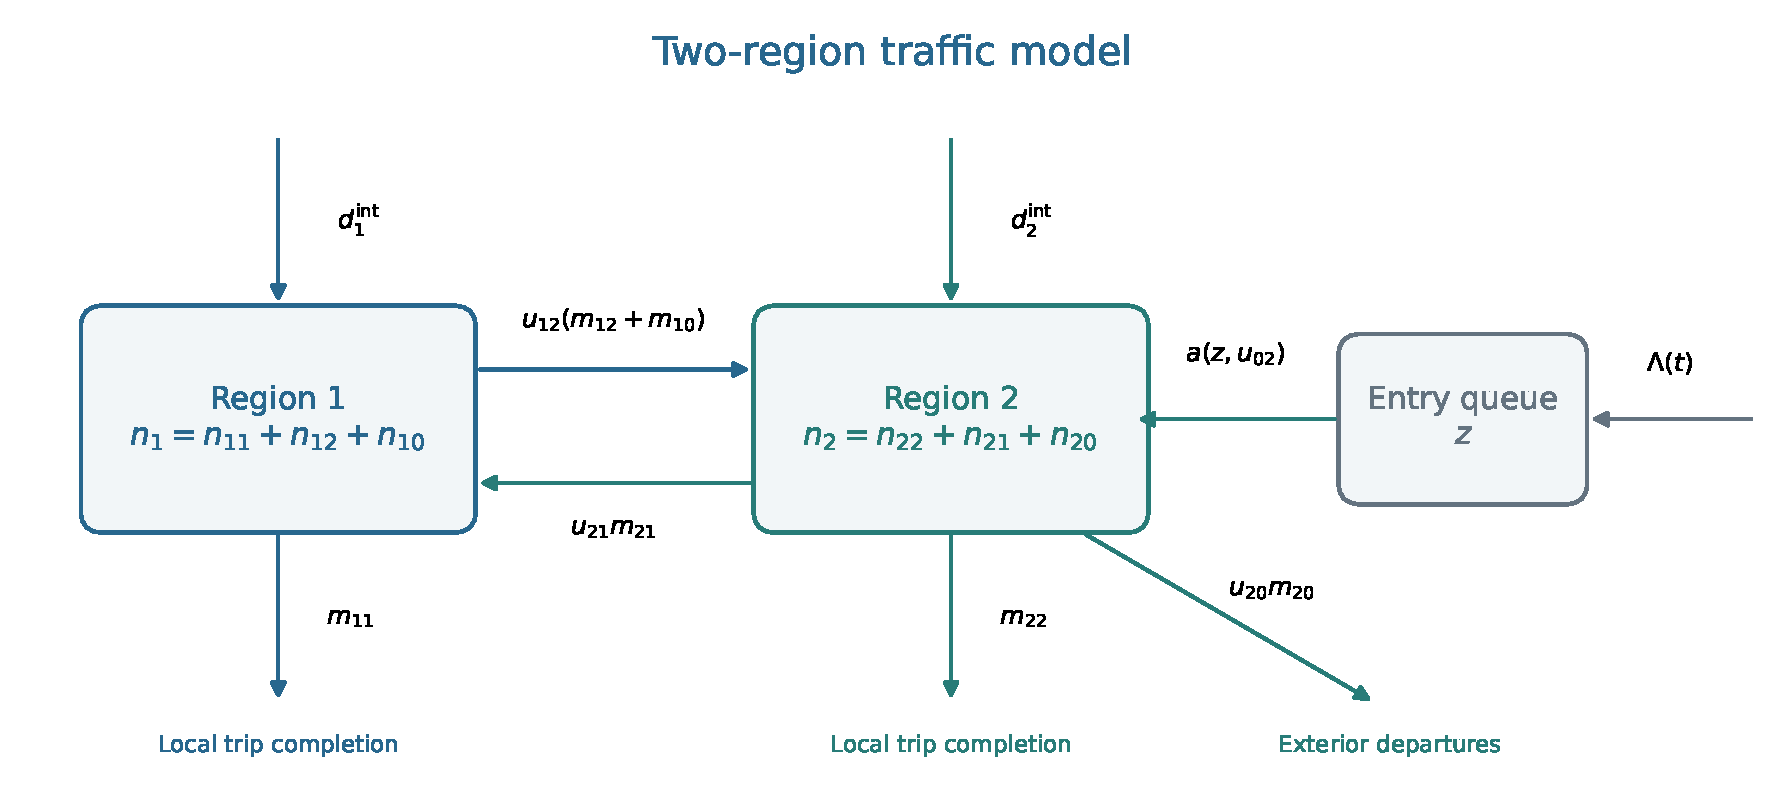
\includegraphics[width=\textwidth]{figures/two_region_vehicle_flows_vector.pdf}
\caption{Two-region traffic model. Regional accumulations $n_1,n_2$ and
the entry queue $z$ are measured in vehicles, and all arrow labels denote
rates in veh/h. Internal demand $d_i^{\rm int}=\sum_j d_{ij}^{\rm int}$
generates trips within Region~$i$, while exterior arrivals $\Lambda(t)$
join the queue. Admission $a(z,u_{02})$ enters Region~2, with fractions
$\pi$ and $1-\pi$ joining $n_{21}$ and $n_{22}$, respectively.
The potential flows $m_{ij}$ are restricted by boundary inputs $u_{ik}$
for transfers and exterior departures. Local trips finish at rates
$m_{11}$ and $m_{22}$. Vehicles retain their final destination when transferring between regions. Destination index $0$ denotes
the exterior.}
\label{fig:two-region-network}
\end{figure}
The regional totals are
\begin{equation}
 n_1=n_{11}+n_{12}+n_{10},\qquad
 n_2=n_{22}+n_{21}+n_{20}.
 \label{eq:regional-class-totals}
\end{equation}
The scalar $z$ is the queue waiting to enter Region~2. Fractions $\pi$
and $1-\pi$ of admission $a$ join vehicles destined for Regions~1
and~2, respectively. Internal demands $d_{ij}^{\rm int}\ge0$ remain
constant in the studies considered here. The scalar arrival error $w$
is bounded in Section~\ref{sec:problem-uncertainty}. With
$\rho_i=n_i/\mathcal L_i$, vehicle conservation gives
\begin{equation}
\begin{aligned}
\dot n_{11}&=-\frac{n_{11}V_1(\rho_1)}{\ell_1}
                 +u_{21}\frac{n_{21}V_2(\rho_2)}{\ell_2}+d_{11}^{\rm int},\\
\dot n_{22}&=-\frac{n_{22}V_2(\rho_2)}{\ell_2}
                 +u_{12}\frac{n_{12}V_1(\rho_1)}{\ell_1}+(1-\pi)a+d_{22}^{\rm int},\\
\dot n_{12}&=-u_{12}\frac{n_{12}V_1(\rho_1)}{\ell_1}+d_{12}^{\rm int},\\
\dot n_{21}&=-u_{21}\frac{n_{21}V_2(\rho_2)}{\ell_2}+\pi a+d_{21}^{\rm int},\\
\dot n_{10}&=-u_{12}\frac{n_{10}V_1(\rho_1)}{\ell_1}+d_{10}^{\rm int},\\
\dot n_{20}&=-u_{20}\frac{n_{20}V_2(\rho_2)}{\ell_2}
                 +u_{12}\frac{n_{10}V_1(\rho_1)}{\ell_1}+d_{20}^{\rm int},\\
\dot z&=\widehat\Lambda+w-a.
\end{aligned}
\label{eq:destination-class-balances}
\end{equation}
The input $u_{12}$ controls both $n_{12}$ and $n_{10}$ vehicles leaving
Region~1 for Region~2. Transfers move $n_{12}$ vehicles into $n_{22}$,
$n_{21}$ vehicles into $n_{11}$, and $n_{10}$ vehicles into $n_{20}$.
The six regional balances follow Mohajerpoor et al.~\cite{mohajerpoor2020hinf},
building on \cite{geroliminis2013mpc,zhong2018robust}. We add the exterior
queue and replace direct gated exterior demand by admission from that
queue. Control inputs may switch between plan blocks, while the
accumulations remain continuous in time.

For queue-release time $\tau_q>0$ and full entrance capacity
$\kappa_{02}>0$, admission is
\begin{equation}
 a(z,u_{02})=\min\{z/\tau_q,\kappa_{02}u_{02}\}.
 \label{eq:new-admission}
\end{equation}
The term $z/\tau_q$ limits admission according to the waiting vehicles,
while $\kappa_{02}u_{02}$ limits it according to the permitted entrance
capacity. This is the single-queue specialization of
\eqref{eq:network-state-space}. Boundary-queue models provide a related
treatment of storage constraints \cite{haddad2017queues}, although here
the queue is outside Region~2 rather than between the two regions.

To retain a specified outflow MFD, the corresponding speed function is
\begin{equation}
 V_i(\rho)=\ell_i\frac{G_i(\mathcal L_i\rho)}{\mathcal L_i\rho}
 \quad(\rho>0),\qquad V_i(0)=\ell_i G_i'(0).
 \label{eq:speed-from-mfd}
\end{equation}
The value at zero uses the differentiable extension with $G_i(0)=0$.
In general, define the regional per-vehicle outflow rate
$v_i(n_i)=V_i(n_i/\mathcal L_i)/\ell_i$, so $m_{ij}=n_{ij}v_i(n_i)$.
The numerical two-region model specializes to identical outflow curves.
For the common two-region curve $G_1=G_2=G$, the calculations use
\begin{equation}
 v(n)=\frac{G(n)}{n}=\frac{V_i(n/\mathcal L_i)}{\ell_i}
 \quad(n>0),\qquad v(0)=G'(0),\qquad m_{ij}=n_{ij}v(n_i).
 \label{eq:per-vehicle-outflow-rate}
\end{equation}
Here $v$ is a per-vehicle outflow rate in h$^{-1}$, while $V_i$ is speed
in km/h. The fitted $v$ is nonnegative and nonincreasing over the
operational range. This representation preserves the given MFD and all
vehicle balances. Physical speed and density scales additionally require
the regional lengths $\ell_i$ and $\mathcal L_i$ to be specified.

The assumptions have distinct roles. Nonnegative speed gives nonnegative
potential outflows and supports the positivity argument. The containment
results require local Lipschitz dynamics and validated bounds on the
retained branch derivatives over each trial region. The nonincreasing
speed assumption describes the traffic model; these proofs do not require
it, or a fixed sign of $G_i'$. The common symbol $v$ in Section~\ref{sec:new-certification}
refers to this fitted two-region specialization. Distinct regional curves
use their own $v_i$ and derivative bounds in the network extension.

\subsection{State representation and physical constraints}
\label{sec:physical-constraints}

A control plan $P$ specifies control inputs or feedback laws over
$[t_0,E]$, from activation at $t_0$ to expiry at $E$. To express the model in the
coordinates used for certification, set
$d_1^{\rm int}=d_{11}^{\rm int}+d_{12}^{\rm int}+d_{10}^{\rm int}$ and
$d_2^{\rm int}=d_{22}^{\rm int}+d_{21}^{\rm int}+d_{20}^{\rm int}$.
Summing the destination-specific balances gives
\begin{equation}
\begin{aligned}
\dot n_1&=d_1^{\rm int}-m_{11}-u_{12}(m_{12}+m_{10})+u_{21}m_{21},\\
\dot n_2&=d_2^{\rm int}-m_{22}+u_{12}(m_{12}+m_{10})-u_{21}m_{21}
             +a-u_{20}m_{20}.
\end{aligned}
\label{eq:regional-flow-balances}
\end{equation}
Collect the regional totals, four destination-specific accumulations, and queue as
\begin{equation}
\begin{aligned}
x&=(n_1,n_2,n_{11},n_{22},n_{10},n_{20},z)^\top,\\
u&=(u_{12},u_{21},u_{02},u_{20})^\top.
\end{aligned}
\label{eq:new-state}
\end{equation}
The other two accumulations are recovered exactly as
$n_{12}=n_1-n_{11}-n_{10}$ and $n_{21}=n_2-n_{22}-n_{20}$.
These coordinates therefore describe the same seven vehicle counts as
\eqref{eq:destination-class-balances}. The dynamics become
\begin{equation}
 \dot x=f(x,u,t)+e_7w(t),\qquad e_7=(0,0,0,0,0,0,1)^\top,
 \label{eq:new-plant}
\end{equation}
where $f$ contains the nominal balances with $w=0$, ordered as in
\eqref{eq:new-state}. Substituting a plan's feedback law into $f$ gives
the block dynamics $f_b$ used in the certification check.

Every plan must satisfy $u(t)\in\mathcal U$ throughout its execution,
where
\begin{equation}
\mathcal U=\{u:0\le u\le1,\ |u_{21}-u_{12}|\le\delta_1^u,
\ |u_{20}-u_{02}|\le\delta_2^u\}.
\label{eq:new-gates}
\end{equation}
The difference bounds follow Mohajerpoor et al.~\cite{mohajerpoor2020hinf}. Opposite-direction
movements can share signal phases, which motivates restricting how far
their aggregate control inputs can differ. The parameters
$\delta_1^u,\delta_2^u\in[0,1]$ specify these operating limits. Each input has the componentwise bounds $[0,1]$, in addition to these
pairwise restrictions. Minimum and maximum green-time bounds, as in
\cite{mohajerpoor2020hinf}, would tighten the componentwise range and
can be represented by the same affine constraints.

Physical feasibility also requires nonnegative destination-specific
accumulations and
\[
0\le n_i\le n_i^{\max}\quad(i=1,2),\qquad 0\le z\le z^{\max}.
\]
The regional bounds are operational accumulation limits, and $z^{\max}$
is exterior storage capacity. Together with \eqref{eq:new-gates}, the
implemented two-region formulation has 24 affine state--input
inequalities. Their numerical limits are given with the experiments.

\subsection{Control objectives and service requirements}
\label{sec:benchmark-formulation}

Control objectives specify the traffic improvement sought from a plan.
The network-efficiency objective minimizes total time spent in both
regions and the exterior queue. For total accumulation
$M=n_1+n_2+z$, its cost is
\begin{equation}
J_Q(P;x_0,w)=\int_{t_0}^{E}M_P(t;x_0,w)\,dt.
\label{eq:benchmark-queue-cost}
\end{equation}
Here
\[
M_P(t;x_0,w)=n_{1,P}(t;x_0,w)+n_{2,P}(t;x_0,w)+z_P(t;x_0,w)
\]
is the total number of vehicles in the two regions and the exterior queue
at time $t$ when plan $P$ is executed from activation state $x_0$ with
arrival error $w$. The subscript $P$ identifies the resulting trajectory.
Costs are measured in vehicle-hours. We suppress $x_0,w$ when they are
fixed or specified by the planning scenario.

A temporary priority for Region~2 is represented by a weight $p\ge1$:
\begin{equation}
J_D(P;x_0,w)=\int_{t_0}^{E}
 \bigl(n_{1,P}(t)+p n_{2,P}(t)+z_P(t)\bigr)\,dt.
\label{eq:benchmark-priority-cost}
\end{equation}
The trajectory components in this expression share the same $x_0,w$.
These objectives express preferences, while service requirements impose
mandatory traffic conditions at specified deadlines:
\begin{equation}
g_r^\top x(T_r)\le\eta_r,\qquad T_r\in[t_0,E].
\label{eq:new-service}
\end{equation}
The dimensionless coefficients $g_r$ select the traffic quantity,
$\eta_r$ is its limit in vehicles, and $T_r$ is its deadline. For example,
$g_r=e_1$, with $e_1$ selecting the first state component, imposes a
Region-1 accumulation limit. Service requirements
remain binding when regional priorities change. Modifying a target or
deadline requires an operator instruction.

The experiments consider a network-efficiency task that minimizes $J_Q$
subject to physical constraints, and a regional-priority task that
minimizes $J_D$ while also requiring $n_1(E)\le\eta$. The cost subscripts Q and D identify the network-efficiency and
regional-priority tasks, respectively. The next subsection specifies the uncertainty under
which their constraints must hold.

\subsection{Uncertainty and feasible plans}
\label{sec:problem-uncertainty}

Consider an activation time $t_0$ at which a bounded state estimate is
available. The framework receives the estimate
$\widehat x_{t_0}$ and a componentwise state-estimation error bound
$d_x\in\mathbb R_{\ge0}^7$ in vehicles. The bound holds simultaneously
for all components. The resulting box is
\begin{equation}
\begin{aligned}
\mathcal I_{t_0}&=\{x:|x-\widehat x_{t_0}|\le d_x\},\\
|w(t)|&\le\bar w,\qquad t\in[t_0,E],
\end{aligned}
\label{eq:benchmark-contract}
\end{equation}
where inequalities are componentwise and $\bar w$ is in veh/h.
Each component of $d_x$ gives the maximum allowed absolute difference
between the corresponding state component and its estimate. These bounds
are the box's \emph{half-widths}. Measurement processing and state estimation
supply the initial estimate and bound externally. Numerical sweeps use a
scalar parameter $d$ to construct $d_x$ as specified for each study.
The forecast $\widehat\Lambda$ and error bound are chosen so that all
allowed arrivals are nonnegative.
\begin{definition}
\label{def:planning-contract}
The \emph{planning contract} is the tuple
\[
\mathcal C=(\mathcal I_{t_0},\bar w,f,\mathcal P_{\rm phys},
\mathcal O,[t_0,E]).
\]
Here $f$ includes the arrival forecast, $\mathcal P_{\rm phys}$ contains
the physical constraints, and $\mathcal O$ contains the service triples
$(T_r,g_r,\eta_r)$ to be met during the execution interval.
\end{definition}
Let $\mathcal W$ contain every measurable arrival error satisfying
\eqref{eq:benchmark-contract}. Write $x_P(s;x_0,w)$ and $u_P(s;x_0,w)$
for the state and applied control at time $s$ under plan $P$.

\begin{definition}
\label{def:robust-feasibility}
Write the physical constraints as $H_jx+J_ju\le\beta_j^{\rm phys}$ and
the service requirements as $g_r^\top x(T_r)\le\eta_r$.
A robustly feasible plan has a well-defined trajectory throughout
$[t_0,E]$ for every allowed initial state and arrival error, and satisfies
all physical constraints throughout this interval and all service
requirements at their deadlines. The set of these plans is
\begin{equation}
\begin{aligned}
\mathcal F_{\mathcal C}=\{P:\;&\forall x_0\in\mathcal I_{t_0},\ w\in\mathcal W,\\
&H_jx_P(s;x_0,w)+J_ju_P(s;x_0,w)\le\beta_j^{\rm phys}\\
&\hspace{1em}\text{for all }s\in[t_0,E]\text{ and physical constraints }j,\\
&g_r^\top x_P(T_r;x_0,w)\le\eta_r
\quad\text{for all service requirements }r\}.
\end{aligned}
\label{eq:benchmark-feasible-set}
\end{equation}
\end{definition}

\begin{definition}
\label{def:feasibility-certificate}
A certification check must accept only robustly feasible plans:
\[
\mathsf{Cert}_{t_0}(P\mid\mathcal C)=1
\quad\Longrightarrow\quad P\in\mathcal F_{\mathcal C}.
\]
Its accepted set therefore satisfies
\begin{equation}
\widehat{\mathcal F}_{\mathcal C}
=\{P:\mathsf{Cert}_{t_0}(P\mid\mathcal C)=1\}
\subseteq\mathcal F_{\mathcal C}.
\label{eq:benchmark-certifiable-set}
\end{equation}
\end{definition}
An inconclusive check leaves robust feasibility undecided. A single
violation under the allowed conditions rules it out.

\paragraph{Problem definition}
\label{prob:supervised-planning}
Given the traffic model, a planning contract, and a sequence of proposed
plans, design a supervisory procedure that performs the following three
functions.
\begin{enumerate}
\item Construct a computable certification procedure satisfying
Definition~\ref{def:feasibility-certificate} and an activation rule that
permits replacement only when a matching certificate is completed by
the activation time.
\item When a proposal is not certified, seek a modified plan that passes
the same check, using a backup certified for the applicable contract.
If no replacement is ready in time, continue the current plan under
its existing certificate.
\item Across successive requests and computation delays, activate a
replacement only when its certificate covers every possible activation
state and every pending service requirement. Otherwise retain
the current plan within its original execution interval.
\end{enumerate}
Planning tools seek low cost under forecast or scenario conditions,
while certification checks the full uncertainty set.

\section{Dual-Agent Planning and Supervisory Control}
\label{sec:new-agent}

\subsection{Architecture overview}
Figure~\ref{fig:new-architecture} separates plan proposal from execution.
The AI agent interprets operator instructions and requests plans from
numerical tools. The rule-based supervisory agent, called the
\emph{supervisor}, checks those plans against independently supplied
traffic information, physical constraints and service requirements.
A deterministic tool interface validates requests and forwards candidates
to both agents; the execution interface applies the supervisor's decision.
Hierarchical perimeter control coordinates decisions across levels
\cite{ramezani2015heterogeneity,su2023hierarchical}. Here the distinction
is between proposing a plan and verifying it before execution. The same
interface accepts proposals from a learned controller, optimizer or human.
Section~\ref{sec:task-state-live} tests an LLM with tool calling.

\begin{figure}[!t]
\centering
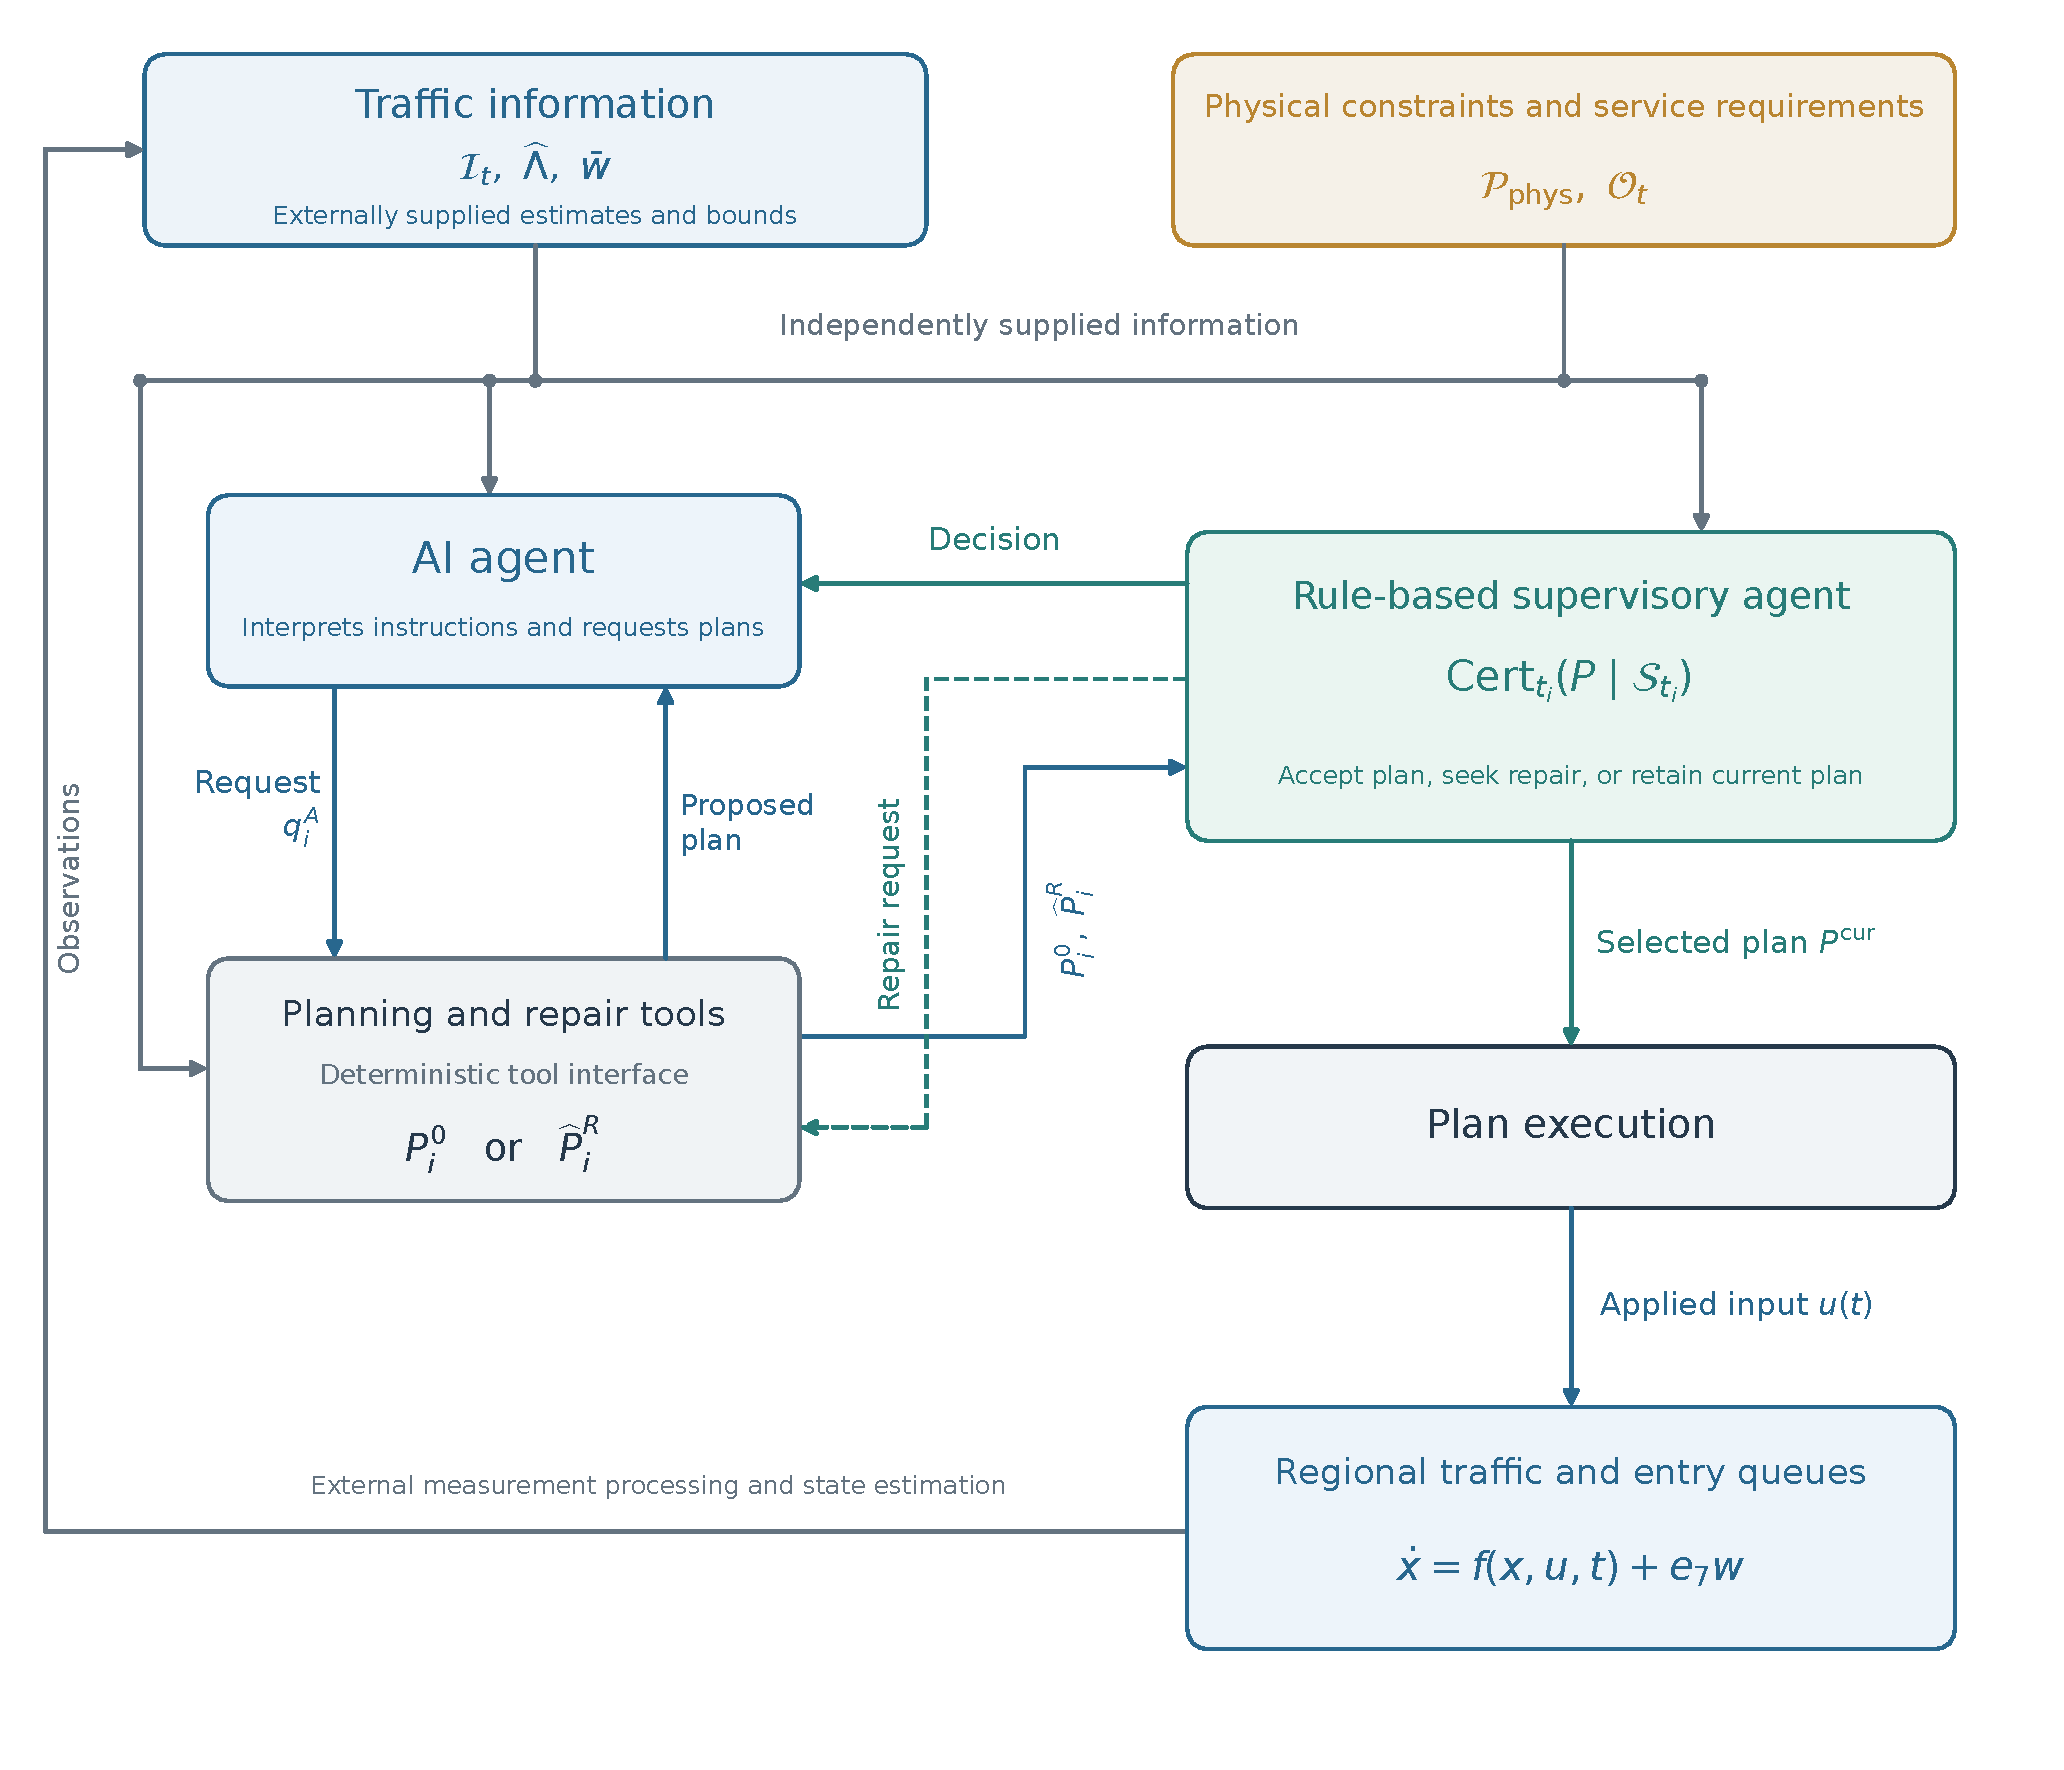
\includegraphics[width=\textwidth]{figures/dual_agent_block_diagram_clarified.pdf}
\caption{Dual-agent architecture. Traffic information comprises the state
set $\mathcal I_t$, arrival forecast $\widehat\Lambda$ and error bound
$\bar w$; physical constraints $\mathcal P_{\rm phys}$ and pending service
requirements $\mathcal O_t$ are supplied independently of the AI agent.
The agent receives summaries and requests plans through $q_i^A$.
Proposals $P_i^0$ and repairs $\widehat P_i^R$ reach both agents, while
the supervisor uses $\mathsf{Cert}$ to select $P^{\rm cur}$ and its
applied input $u(t)$. Dashed requests indicate automatic repair.
Observations return to the external estimation process. Feedback plans
require the state access specified in Section~\ref{sec:control-plans}.}
\label{fig:new-architecture}
\end{figure}

\subsection{Control plans}
\label{sec:control-plans}
A plan specifies a control law on each of $N_b$ blocks:
\begin{equation}
\begin{aligned}
P&=\bigl((\tau_b,\tau_{b+1},k_b,K_b)\bigr)_{b=0}^{N_b-1},
\qquad t_0=\tau_0<\cdots<\tau_{N_b}=E,\\
u_P(t)&=k_b+K_bx(t),\qquad t\in[\tau_b,\tau_{b+1}).
\end{aligned}
\label{eq:control-plan-tuple}
\end{equation}
The last block supplies the left-limit input at expiry $E$ unless a
certified successor starts there. States remain continuous at input
changes, and constraints are checked on both sides. Target feedback
$u=u_b^\star+K_b(x-x_b^\star)$ corresponds to
$k_b=u_b^\star-K_bx_b^\star$. For $K_b\ne0$, execution assumes access to
the true state. Activation uncertainty is covered by the initial set;
feedback from estimates would require additional input-error bounds.

With $K_b=0$, the plan is an open-loop, piecewise-constant schedule.
The MPC tool solves a finite-horizon problem when requested, without
automatic receding-horizon updates \cite{geroliminis2013mpc}. A schedule
continues until replacement or expiry. Its certificate covers $[t_0,E]$;
operation beyond $E$ requires a certified replacement or a verified
terminal policy, as specified in \appref{sec:terminal-backup}.

\subsection{AI agent and planning tools}
\label{sec:agent-requests}
At request time $t_i^{\rm req}$, the agent receives instructions, traffic
and requirement summaries, and its interaction history: earlier
instructions, tool responses and supervisory feedback. Memory is a stored
summary of this history. Planning tools return candidate plans for a
requested objective; the repair tool searches for a modified candidate.

The history-only format supplies these inputs directly. The task-record
format additionally supplies $\theta_i$, containing the active priority,
absolute expiry $T^{\rm prio}$ and interrupted priorities. The compiler
$\mathsf{Comp}$ validates the operation, updates $\theta_i$ using
Table~\ref{tab:task-operations}, and forms $q_i^A$ with the objective,
remaining duration and cost weights. Invalid requests give $q_i^A=\bot$.
Interrupted priorities retain their absolute expiries, and priority
changes leave pending service requirements unchanged.

Repair can be invoked automatically by the supervisor after rejection
or requested by the agent following feedback. Section~\ref{sec:new-incident-protocol}
uses the automatic mode; Section~\ref{sec:task-state-live} uses
agent-requested repair and compares the two input formats. Both modes
use the same certification and activation rules.

\subsection{Supervisory agent}
\label{sec:supervisory-agent}
A certificate records the checked plan, contract, execution interval and
verified state bounds. It matches execution when the coefficients,
activation time, model and data versions, and authorized requirements
agree, and its state and arrival sets cover the execution uncertainty.
The supervisor stores
\[
\mathcal S_t=(\mathcal I_t,\mathcal W_t,\mathcal O_t,
P_t^{\rm cur},\mathcal H_t,P_t^B,t,\mathsf{ver}_t).
\]
Here $\mathcal I_t$ is the supplied or propagated state set,
$\mathcal W_t$ the arrival-error family, and $\mathcal O_t$ the accepted
service requirements whose deadlines have not passed. The current plan
$P_t^{\rm cur}$ retains its original certificate $\mathcal H_t$, expiry
$E_{\rm cur}$ and reachable sets, including all component certificates
when the initial set is subdivided. The identifier $\mathsf{ver}_t$
records model, forecast, physical-constraint and service-requirement
versions, including deadline changes. The repair backup is $P_t^B$, or
$\bot$ when unavailable. These fields and a candidate expiry $E$ define
$\mathcal C(\mathcal S_t,E)$ in Definition~\ref{def:planning-contract}, so
$\mathsf{Cert}_t(P\mid\mathcal S_t)$ abbreviates
$\mathsf{Cert}_t(P\mid\mathcal C(\mathcal S_t,E))$.

When repair is invoked,
\begin{equation}
\widehat P_i^R=\mathsf{RepairTool}
(P_i^0,P_i^B,\mathcal S_{t_i},\mathcal G_{\rm rep}).
\label{eq:repair-tool-interface}
\end{equation}
The backup must pass under the same conditions as the candidates. It may
be the remaining current plan, rechecked for that contract, or a newly
certified plan. It is distinct from the terminal policy beyond expiry.
Section~\ref{sec:predictive-repair} defines the search; Algorithm~\ref{alg:agent-execution}
governs activation of both original and repaired proposals.

\begin{remark}
Failure to recertify the current plan from an enlarged state set does not
invalidate its original certificate. While its original assumptions hold,
that schedule and certificate remain usable until expiry or replacement.
\end{remark}

\subsection{Timing, assumptions, and execution}
\label{sec:execution-interface}
Requests occur at $t_i^{\rm req}\le t_i$, where $t_i$ is the possible
activation time and $t_{\rm ready}$ is certificate completion time.
The index $i$ on $t_i$, $\mathcal I_i=\mathcal I_{t_i}$,
$\mathcal S_{t_i}$, $P_i$, $\theta_i$ and $q_i^A$ denotes a decision;
indices on traffic variables retain their regional or boundary meaning.
Traffic evolves continuously during computation, service deadlines keep
their absolute times, and only finitely many decisions occur on a finite
interval. Certification relies on the following external and interface
conditions.

\begin{assumption}
\label{ass:trusted-inputs}
Each externally supplied state set contains the actual state at its
timestamp, the stated arrival-error bounds hold, and traffic follows
\eqref{eq:new-plant} under the model and uncertainty assumptions of the
active certificate. Physical constraints and service requirements are
authorized by the operator. These data reach the tools and supervisor
independently of agent requests and memory.
\end{assumption}

\begin{assumption}
\label{ass:supervisory-separation}
The execution interface satisfies the following conditions:
\begin{enumerate}
\renewcommand{\labelenumi}{(\alph{enumi})}
\item Agent outputs cannot modify independently supplied data, pending
requirements, or the decision record.
\item Only the supervisor authorizes activation, and execution uses the
checked coefficients, timing, and model version.
\item A new service requirement becomes pending only when the selected
plan covers it.
\item Invalid requests, failed checks, and late results leave the current
plan and its original certificate in use, while their assumptions hold,
until expiry or a later certified replacement.
\end{enumerate}
\end{assumption}

The guarantee concerns physical constraints and service requirements;
correct interpretation of the requested objective is evaluated separately.

\begin{algorithm}[!htbp]
\caption{Planning requests and certified execution}
\label{alg:agent-execution}
\begin{minipage}{\linewidth}
\small
\textbf{Input:} current certified plan and record $\mathcal S_t$,
operator requests, independently supplied traffic data and requirements,
agent history, and $\theta_i$ when used.\\
\textbf{Output:} selected plan and certificate, updated record and feedback.\\
For each request at $t_i^{\rm req}$, while the current plan remains in force:
\begin{enumerate}
\setlength{\itemsep}{2pt}
\item \label{step:request}\textbf{Interface and agent:} process priority
expiries and form $q_i^A$, using $\mathsf{Comp}$ for the task-record
variant or direct validation otherwise. If $q_i^A=\bot$, retain the
current decision record and return feedback.
\item \label{step:planning}\textbf{Planning tool:} use $q_i^A$ and the
independent data to generate $P_i^0$. The interface forwards it to the
supervisor and returns plan information to the agent.
\item \label{step:activation}\textbf{Supervisor:} choose $t_i$ and
assemble $\mathcal S_{t_i}$ from a propagated containing state set or a
valid estimate at activation (Proposition~\ref{prop:planned-handover}).
Preserve accepted deadlines, including those during computation.
\item \label{step:checking}\textbf{Supervisor and repair tool:} apply
$\mathsf{Cert}_{t_i}(P_i^0\mid\mathcal S_{t_i})$ using
Theorem~\ref{thm:new-plan-enclosure} and, when used,
Proposition~\ref{prop:structure-plan}. Portfolio checks use the complete-cover
rule \eqref{eq:portfolio-cover-rule}. After rejection, invoke repair only
if requested by the agent or enabled automatically. Check every repair
and its backup under the same conditions.
\item \label{step:installation}\textbf{Supervisor:} activate only when
the matching certificate is complete by $t_i$, execution data match, and
all pending requirements are covered. Otherwise retain the current plan,
certificate and expiry. Accept a new service requirement only when the
selected plan covers it.
\item \label{step:feedback}\textbf{Interface:} return feedback, update
history and the decision record, and execute within the selected plan's
certified interval.
\end{enumerate}
\end{minipage}
\end{algorithm}
\FloatBarrier

\section{Runtime Certification Using Traffic Structure}
\label{sec:new-certification}


This section constructs the certification procedure used in
Step~\ref{step:checking} of Algorithm~\ref{alg:agent-execution}. It first
bounds the states reached under one plan, then uses those bounds to
justify replacement, repair and delayed activation. The bounds use coordinate choices,
nonnegativity, independent queue comparisons and shared uncertainty.
The proofs combine validated numerics \cite{tucker2011validated},
generalized Jacobians \cite{clarke1990optimization}, and comparison
arguments \cite{khalil2002nonlinear,farina2000positive}.
\appref{sec:terminal-backup} gives terminal-continuation conditions, and
\appref{sec:repair-cost-bound} gives a conditional repair-cost bound.

\subsection{Plan data and coordinate choices}

For each block of a plan defined in Section~\ref{sec:control-plans},
the certification procedure uses the control law and arrival uncertainty
\begin{equation}
 u_b(x)=k_b+K_bx,
 \qquad \Lambda(t)=\widehat\Lambda(t)+w(t),
 \qquad |w(t)|\le\bar w.
 \label{eq:new-plan-data}
\end{equation}
The forecast is continuous and piecewise affine; $w$ is any measurable
signal satisfying the bound. Feedback uses the exact state as specified
in Section~\ref{sec:control-plans}.

For the physical constraints in Definition~\ref{def:robust-feasibility},
substitution of the block law gives
\begin{equation}
 h_{jb}^\top x\le\beta_{jb},\qquad
 h_{jb}^\top=H_j+J_jK_b,\qquad
 \beta_{jb}=\beta_j^{\rm phys}-J_jk_b.
 \label{eq:new-physical-rows}
\end{equation}
Here $j=1,\ldots,n_c$ indexes physical constraints. The service
requirements remain $g_r^\top x(T_r)\le\eta_r$ for $r=1,\ldots,n_s$,
as in \eqref{eq:new-service}. Each two-sided input-difference bound in
\eqref{eq:new-gates} contributes two physical inequalities.

The network model first gives a coordinate construction independent of
its number of regions. Write $F(c,u,t)=d^{\rm int}(t)+B(u)m(c)$, so
$\dot c=F(c,u,t)+P_a a$ and $\dot z=\Lambda-a$, with fixed $P_a$ and
$\mathbf1^\top P_a=\mathbf1^\top$.

The following proposition isolates admission in the queue coordinates
while counting every internal and waiting vehicle exactly once.

\begin{proposition}
\label{prop:network-localization}
For fixed $P_a$, the invertible coordinate map
\begin{equation}
 L_a=\begin{bmatrix}I&P_a\\0&I\end{bmatrix},\qquad
 y=L_a\begin{bmatrix}c\\z\end{bmatrix}
   =\begin{bmatrix}c+P_a z\\z\end{bmatrix}
 \label{eq:network-transform}
\end{equation}
gives
\begin{equation}
 \dot y_c=F(y_c-P_a z,u,t)+P_a\Lambda,\qquad
 \dot z=\Lambda-a.
 \label{eq:network-transformed-flow}
\end{equation}
Thus explicit admission terms occupy only the $n_q$ queue coordinates. No
invertible linear transformation can confine these $n_q$ independent channels
to fewer than $n_q$ scalar coordinates. Moreover,
$\mathbf1_{n_{\rm acc}}^\top y_c=\mathbf1_{n_{\rm acc}}^\top c+\mathbf1_{n_q}^\top z$, so the combined
accumulations count all internal and waiting vehicles exactly once.
\end{proposition}

\begin{proof}
The inverse is $c=y_c-P_a z$. Differentiation and the admission
incidence give
\[
\dot y_c=F(c,u,t)+P_a a+P_a(\Lambda-a)=F(c,u,t)+P_a\Lambda,
\qquad
L_a\begin{bmatrix}P_a\\-I\end{bmatrix}=\begin{bmatrix}0\\-I\end{bmatrix}.
\]
The original incidence has rank $n_q$ because of its lower block $-I$.
An invertible map preserves rank, while support on fewer than $n_q$ rows
would lower it. Finally, $\mathbf1^\top P_a=\mathbf1^\top$ gives the
stated total-accumulation identity.
\end{proof}

Recovering the six destination accumulations from the two-region state
$x$ and applying Proposition~\ref{prop:network-localization} gives

\begin{equation}
\begin{aligned}
y=Lx=(&n_{11},n_{12},n_{10},n_{22}+(1-\pi)z,\\
      &n_{21}+\pi z,n_{20},z)^\top.
\end{aligned}
\label{eq:new-conservation-coordinates}
\end{equation}
Admitting a vehicle transfers it from the queue into the region without
changing the corresponding combined quantity. The transformation is
invertible, with
\begin{equation}
 \begin{aligned}
 n_1&=y_1+y_2+y_3,&n_2&=y_4+y_5+y_6-y_7,\\
 n_{11}&=y_1,&n_{22}&=y_4-(1-\pi)y_7,\\
 n_{10}&=y_3,&n_{20}&=y_6,\qquad z=y_7.
 \end{aligned}
 \label{eq:new-inverse-coordinates}
\end{equation}
For admission incidence $b_a=(0,1,0,1-\pi,0,0,-1)^\top$,
\begin{equation}
 Lb_a=-e_7,
 \qquad Le_7=(0,0,0,1-\pi,\pi,0,1)^\top.
 \label{eq:new-conservation-incidence}
\end{equation}
Thus $n_1+n_2+z=\sum_{i=1}^6y_i$, and admission cancels from the
combined accumulations. For example,
\[
\frac{d}{dt}(n_{21}+\pi z)
=d_{21}^{\rm int}-u_{21}m_{21}+\pi\Lambda.
\]
This cancellation avoids bounding the same uncertain admission twice
with opposite signs. Regional outflow still depends on the transformed
state, and the queue remains necessary to recover regional accumulations.

Coordinate choice depends on the verified admission branch. Queue-limited
admission depends on uncertain $z$, so conservation coordinates remove
that shared term, although arrival error still enters through $Le_7w$.
Under capacity-limited constant inputs, $a=\kappa_{02}u_{02}$ is independent
of $z$, and the regional equations are independent of arrival error.
Destination coordinates
\[
\widetilde Lx=(n_{11},n_{12},n_{10},n_{22},n_{21},n_{20},z)^\top
\]
preserve this separation. Neither representation dominates in general.

The containment proofs apply to any fixed invertible $L$ retaining $z$
as its last coordinate, with the Jacobian, disturbance, predictor and
constraint bounds recomputed accordingly. This also preserves the scalar
queue intersection below. Branch exclusions must hold over the entire
predictor-to-state segment, not just the nominal trajectory.

A finite portfolio can test these fixed transforms on either the full
initial set or a prescribed subdivision. For a configuration $\mathsf k$, let
$\mathcal I_{t_0}\subseteq\bigcup_{j=1}^{N_{\rm box}(\mathsf k)}\mathcal I_{\mathsf k,j}$ be a finite cover,
and require the same plan, uncertainty bounds, physical limits and service
requirements for every member. Its acceptance rule is
\begin{equation}
 \operatorname{Cert}^{\rm port}(P\mid\mathcal C)=1
 \quad\Longleftrightarrow\quad
 \exists\mathsf k\ \forall j:\
 \operatorname{Cert}_{\mathsf k,j}(P\mid\mathcal C_{\mathsf k,j})=1,
\label{eq:portfolio-cover-rule}
\end{equation}
where $\mathcal C_{\mathsf k,j}$ changes only the initial set to
$\mathcal I_{\mathsf k,j}$. Outward-rounded members may extend beyond
the original set. Every allowed initial state lies in a member whose
certificate establishes the constraints, so a complete passing
configuration proves correctness. Incomplete configurations are not
combined. The numerical order is unsplit conservation, unsplit destination,
four-box destination, then four-box conservation, fixed before checking
the candidate. The activation rule still requires timely completion.

\subsection{Certification of one plan}
\label{app:new-enclosure-proof}

Let $f_b$ be the nominal field on control block $b$, so the actual field
is $f_b(x,t)+e_7w$. The fitted outflow and affine admission branches give
a locally Lipschitz state field, measurable in time. Bounded measurable
arrival errors therefore admit unique local absolutely continuous
solutions. The polynomial extends to trial sets outside the physical
domain, while accepted trajectories must satisfy its constraints.
No fixed sign of $G_i'$ is required, so the construction includes the
congested branch.

Partition the plan at control changes, forecast-slope changes, service
deadlines and prediction checkpoints. On $[t_l,t_l+h_l]$, a differentiable
predictor $\mathbf p_l$ and inherited radius $r_l\ge0$ satisfy
$|L(x(t_l)-\mathbf p_l(t_l))|\le r_l$. Initially, $r_0\ge|L|d_x$ covers
the physical box centered at $\mathbf p(t_0)$. The trial set
$\mathbf p_l(t)+L^{-1}[-R_l,R_l]$, $R_l>0$, is the proposed continuous
enclosure. Local time $s$ means absolute time $t_l+s$. The implementation
uses a quadratic predictor from the nominal field, Jacobian and forecast
slope; the bounds include its derivative mismatch. Over the entire
trial set and interval, obtain

\begin{equation}
 \begin{aligned}
 a_{il}^{\rm cmp}&\ge\sup (L D_xf_b L^{-1})_{ii},\\
 b_{ijl}^{\rm cmp}&\ge\sup |(L D_xf_b L^{-1})_{ij}|\quad(j\ne i),\\
 \delta_{il}&\ge\sup_t |(L f_b(\mathbf{p}_l(t),t)-L\dot{\mathbf{p}}_l(t))_i|.
 \end{aligned}
 \label{eq:new-local-bounds}
\end{equation}
At an admission-branch boundary, the generalized Jacobian lies in the
convex hull of the smooth branch limits. Include both branches unless
verified bounds exclude one over the whole trial set. Comparison
coefficients (superscript $\mathrm{cmp}$) retain diagonal signs and bound
off-diagonal magnitudes. Define

\begin{align}
 c_{il}^{\rm cmp}(R_l)&=\sum_{j\ne i}b_{ijl}^{\rm cmp}R_{jl}
                  +\delta_{il}+|(Le_7)_i|\bar w,\nonumber\\
 \phi_{il}(s)&=e^{a_{il}^{\rm cmp}s}r_{il}
                   +\chi(a_{il}^{\rm cmp},s)c_{il}^{\rm cmp}(R_l),\nonumber\\
 \chi(\mu,s)&=\begin{cases}(e^{\mu s}-1)/\mu,&\mu\ne0,\\s,&\mu=0.\end{cases}
 \label{eq:new-component-comparison}
\end{align}
Containment and continuous physical feasibility pass when
\begin{align}
 \max\{r_{il},\phi_{il}(h_l)\}&<R_{il}\quad\text{for every }i,
 \label{eq:new-self-inclusion}\\
 \sup_{t\in[t_l,t_l+h_l]}h_{jb}^\top \mathbf{p}_l(t)
       +|h_{jb}^\top L^{-1}|R_l&\le\beta_{jb}.
 \label{eq:new-affine-support}
\end{align}
The strict self-inclusion check keeps the error inside the trial set;
the support bound verifies every physical constraint throughout the
interval. Absolute values are componentwise. Recenter at a new predictor
using

\begin{equation}
 \delta^{\rm rec}_l\ge
 |L(\mathbf{p}_l(t_{l+1})-\mathbf{p}_{l+1}(t_{l+1}))|,
 \label{eq:new-recentering-bound}
\end{equation}
and propagate $r_{i,l+1}=\phi_{il}(h_l)+\delta^{\rm rec}_{il}$. At a service checkpoint, the paired predictor center $\mathbf p(T_r)$
and inherited radius $r(T_r)$ give
\begin{equation}
 g_r^\top\mathbf p(T_r)+|g_r^\top L^{-1}|r(T_r)\le\eta_r.
 \label{eq:new-service-support}
\end{equation}

At control changes, also check successor-input constraints on the
inherited box. These tests give the following one-plan guarantee.

\begin{theorem}
\label{thm:new-plan-enclosure}
Consider the MFD field \eqref{eq:new-plant} with admission
\eqref{eq:new-admission}, a finite affine-feedback plan implemented as
$u(t)=u_b(x(t))$, and the uncertainty
class \eqref{eq:new-plan-data}. Let its initial information set be contained
in the initial predictor box. Suppose the bounds
\eqref{eq:new-local-bounds} hold for every state and time in each trial
region, and
\eqref{eq:new-self-inclusion} holds on every interval. Then the propagated
boxes contain every trajectory from that initial set under every allowed
arrival error. If \eqref{eq:new-affine-support} and
\eqref{eq:new-service-support} also pass, the trajectory satisfies every
physical constraint continuously through the plan's expiry and every included
service requirement at its deadline, including the successor-input
constraints checked at block boundaries.
\end{theorem}

\begin{proof}
On one interval, omit $l$ and set $z_e=L(x-\mathbf p)$.
Initially $|z_e|\le r<R$. Before a component first reaches its trial
radius, the predictor-to-state segment lies in the trial set. The
locally Lipschitz mean-value relation \cite{clarke1990optimization} gives
\begin{equation}
\dot z_e=A^{\rm mv}(t)z_e+\epsilon(t)+(Le_7)w(t),
\label{eq:new-error-dynamics}
\end{equation}
almost everywhere, where $\epsilon=Lf_b(\mathbf p,t)-L\dot{\mathbf p}$
and $|\epsilon_i|\le\delta_i$. The mean-value
matrix is a weighted average of transformed branch Jacobians, so
$A_{ii}^{\rm mv}\le a_i^{\rm cmp}$ and
$|A_{ij}^{\rm mv}|\le b_{ij}^{\rm cmp}$. Therefore
\begin{equation}
\dot e_i^{\rm abs}\le a_i^{\rm cmp}e_i^{\rm abs}+c_i^{\rm cmp}(R),
\qquad e_i^{\rm abs}=|(z_e)_i|,
\label{eq:new-error-comparison-proof}
\end{equation}
almost everywhere, including at zero components. Multiplying by
$e^{-a_i^{\rm cmp}s}$ and integrating gives
$e_i^{\rm abs}(t_l+s)\le\phi_i(s)$. Since
$\phi_i'(s)=e^{a_i^{\rm cmp}s}(a_i^{\rm cmp}r_i+c_i^{\rm cmp}(R))$
has constant sign, its maximum is
$\max\{r_i,\phi_i(h)\}<R_i$. Continuity excludes a first boundary
contact. Local regularity and the bounded enclosure permit continuation
to the endpoint.

State continuity and \eqref{eq:new-recentering-bound} give
\[
|L(x(t_{l+1})-\mathbf p_{l+1}(t_{l+1}))|
\le\phi(h)+\delta_l^{\rm rec}=r_{l+1}.
\]
Induction proves containment. Substituting $x=\mathbf p+L^{-1}z_e$
gives the physical support bound
$h_{jb}^\top x\le h_{jb}^\top\mathbf p+|h_{jb}^\top L^{-1}|R$;
\eqref{eq:new-affine-support} checks its time maximum. The inherited
endpoint box gives \eqref{eq:new-service-support} and checks successor
inputs. Hence every physical constraint and scheduled service requirement
holds on its specified interval or deadline.
\end{proof}


Every acceptance bound includes numerical rounding error.
\appref{app:verified-arithmetic} gives the outward-rounding rules and
exact checks for constant control inputs.

\subsection{Traffic structure and tighter bounds}
\label{sec:structure-certificate}
\label{app:structure-proof}

For constant inputs, nonnegative accumulations, independent queue bounds
and shared initial uncertainty can sharpen the preceding checks.

\paragraph{Nonnegative destination-specific accumulations}
The balances for the two derived accumulations are
\begin{equation}
 \begin{aligned}
 \dot n_{12}&=d^{\rm int}_{12}-u_{12}v(n_1)n_{12},\\
 \dot n_{21}&=d^{\rm int}_{21}+\pi a-u_{21}v(n_2)n_{21}.
 \end{aligned}
 \label{eq:structure-derived-classes}
\end{equation}
For a quadratic per-vehicle outflow rate
$v(n)=\alpha_2n^2+\alpha_1n+\alpha_0$, the sufficient conditions
$\alpha_2>0$ and $4\alpha_2\alpha_0-\alpha_1^2>0$ give
\begin{equation}
 v(n)=\alpha_2\left(n+\frac{\alpha_1}{2\alpha_2}\right)^2+
                    \frac{4\alpha_2\alpha_0-\alpha_1^2}{4\alpha_2}>0.
 \label{eq:structure-positive-factor}
\end{equation}
The fitted coefficients satisfy these conditions. More generally,
the result needs $v\ge0$, or $V_i(\rho_i)/\ell_i\ge0$, and allows
both increasing and decreasing regional outflow.

\paragraph{Independent queue bounds}
With constant control inputs, the queue depends on its own accumulation and
the exterior arrival rate, so it can be bounded before the coupled
regional states. It satisfies the scalar equation
\begin{equation}
 \dot z=\widehat\Lambda(t)+w(t)-\min\{z/\tau_q,\kappa_{02}u_{02}\}.
 \label{eq:structure-scalar-queue}
\end{equation}
Extreme initial queues and arrival bounds define lower and upper
comparison solutions. Write $\bar a=\kappa_{02}u_{02}$ for the constant
admission capacity set by the entrance input. For constant exterior arrival
$\Lambda_*$, each branch has the solution
\begin{equation}
 \begin{aligned}
 z(s)&=\tau_q\Lambda_*+(z_0-\tau_q\Lambda_*)e^{-s/\tau_q}
       &&(z/\tau_q\le\bar a),\\
 z(s)&=z_0+(\Lambda_*-\bar a)s&&(z/\tau_q\ge\bar a).
 \end{aligned}
 \label{eq:structure-queue-flows}
\end{equation}
The branches join at $z=\tau_q\bar a$. Verified exponential and logarithmic
evaluation bounds their crossing times. When a common branch has not
been established over a forecast interval, its extremal exterior arrivals
give continuous queue bounds. When those bounds establish one branch throughout the
interval and the forecast is $\Lambda_0+\Lambda_1s$, sharper endpoints are
\begin{equation}
\begin{aligned}
 z(h)&=e^{-h/\tau_q}z_0+(\Lambda_0\pm\bar w)\varphi_1+\Lambda_1\varphi_2
       &&\text{(queue-limited)},\\
 z(h)&=z_0+(\Lambda_0\pm\bar w-\bar a)h+\Lambda_1h^2/2
       &&\text{(capacity-limited)},\\
 \varphi_1&=\tau_q(1-e^{-h/\tau_q}),\qquad
 \varphi_2=\tau_q(h-\varphi_1).
\end{aligned}
\label{eq:structure-affine-queue}
\end{equation}
The minus and plus signs give lower and upper solutions. These sharpen
the endpoint bound while the established continuous enclosure remains
in force. Initial physical boxes must satisfy destination-specific and queue
nonnegativity. Subsequent endpoint sets may be intersected with these
independent bounds and then enclosed outward, including recentering error.

\paragraph{Shared initial uncertainty}
To preserve dependence on the uncertain initial state, write

\begin{equation}
 \begin{aligned}
 L(x-\mathbf{p}_l)&=\Gamma_l(s)\xi+\zeta_l(s),\qquad |\xi|\le\mathbf1,\\
 \Gamma_l(s)&=e^{A_l^0s}\Gamma_l(0),\qquad |\zeta_l(0)|\le r_l^{\rm rem}.
 \end{aligned}
 \label{eq:structure-affine-set}
\end{equation}
The shared vector $\xi$ remains fixed across intervals. The columns of
$\Gamma_l$ are signed generators; their box image is a zonotope.
Propagation by $A_l^0$ retains dependencies lost by repeated boxing
\cite{kochdumper2021sparse}. The remainder $\zeta_l$ contains unrepresented
effects and may depend on $\xi$. Initially, a physical box gives
$\mathbf p(t_0)=\widehat x$, $\Gamma(0)=L\operatorname{diag}(d_x)$ and
$r^{\rm rem}=0$, with numerical conversion error added outward.
For the mean-value matrix $A_l^{\rm mv}$ and residual
$\epsilon_l=Lf_b(\mathbf p_l,t)-L\dot{\mathbf p}_l$, differentiation gives

\begin{equation}
 \begin{aligned}
 \dot\zeta_l={}&A_l^{\rm mv}(s)\zeta_l+(A_l^{\rm mv}(s)-A_l^0)\Gamma_l(s)\xi\\
              &+\epsilon_l+(Le_7)w.
 \end{aligned}
 \label{eq:structure-remainder-identity}
\end{equation}
Every Jacobian bound must cover the full predictor-to-true-state segment.
For the queue coordinate, intersect the original trial enclosure with the
convex hull of predictor queue values and independent continuous true-queue
bounds. This retains the segment even when the predictor lies outside the
true queue range. A branch may be excluded only throughout this restricted
enclosure.

Omit $l$, and let $\mathcal J_\varpi$ contain the retained transformed branch
Jacobians. We construct a matrix with nonnegative off-diagonal entries (a Metzler
matrix) to compare componentwise error bounds \cite{farina2000positive}. This matrix and the bound
on the remaining forcing terms are
\begin{equation}
 \begin{aligned}
 \overline{M}_{ii}&=\max_\varpi\sup(\mathcal J_\varpi)_{ii},\\
 \overline{M}_{ij}&=\max_\varpi\sup|(\mathcal J_\varpi)_{ij}|\quad(i\ne j),\\
 (b_\zeta)_i&\ge\max_\varpi\sup_{A_{\rm loc}\in\mathcal J_\varpi,\,\widetilde\Gamma\in\mathcal G_\Gamma}
                  \sum_j|[(A_{\rm loc}-A^0)\widetilde\Gamma]_{ij}|\\
             &\hspace{1em}+\delta_i+|(Le_7)_i|\bar w,
 \end{aligned}
 \label{eq:structure-metzler}
\end{equation}
where $\mathcal G_\Gamma$ contains every $e^{A^0s}\Gamma(0)$ on $[0,h]$ and
$\delta_i\ge\sup_s|\epsilon_i(s)|$. The remainder comparison is
\begin{equation}
 |\zeta(s)|\le e^{\overline{M}s} r^{\rm rem}+\Psi(s)b_\zeta,
 \qquad \Psi(s)=\int_0^s e^{\overline{M}\tau}\,d\tau.
 \label{eq:structure-remainder-bound}
\end{equation}
The exponential is nonnegative and $\Psi$ is componentwise increasing.
Individual entries of the exponential may decrease, so the inherited
remainder must be bounded over the full interval. The outward bounds are
\begin{equation}
 \begin{aligned}
 r_i^{\rm gen}&\ge\sup_{s\in[0,h]}\sum_j|(e^{A^0s}\Gamma(0))_{ij}|,\\
 r_i^\zeta&\ge\sup_{s\in[0,h]}(e^{\overline{M}s} r^{\rm rem})_i
                            +(\Psi(h)b_\zeta)_i.
 \end{aligned}
 \label{eq:structure-continuous-radii}
\end{equation}
Strict containment requires $r^{\rm gen}+r^\zeta<R$. For any constraint
$a_x^\top x\le b_x$, its continuous maximum is bounded by
\begin{equation}
 \sup_s a_x^\top \mathbf{p}(s)+
 \sup_s\|a_x^\top L^{-1}e^{A^0s}\Gamma(0)\|_1+
 |a_x^\top L^{-1}|r^\zeta.
 \label{eq:structure-signed-output}
\end{equation}
The signed constraint coefficients are combined before taking absolute
values, preserving cancellations between state errors that share the same uncertainty. At a
scheduled endpoint use the endpoint generator and remainder. Independently established nonnegativity and queue bounds, together with
exact checks of constant control inputs, may verify the corresponding
constraints. Each constraint can therefore use its tighter valid bound.

Let $\widehat\Gamma$ be the stored endpoint generator and let $d_\Gamma$
bound the row sums of $|e^{A^0h}\Gamma(0)-\widehat\Gamma|$.
The predictor-center change in \eqref{eq:new-recentering-bound} gives
the remainder update
\begin{equation}
 (r^{\rm rem})^+\ge d_\Gamma+e^{\overline{M}h} r^{\rm rem}+\Psi(h)b_\zeta+\delta^{\rm rec}.
 \label{eq:structure-endpoint-update}
\end{equation}
The same $\xi$ is retained. The total queue error combines generator and
remainder terms that may cancel, so a bound on their sum cannot be applied
separately to either term.

The next proposition verifies that these traffic-specific refinements
also establish the containment in \eqref{eq:benchmark-certifiable-set}.

\begin{proposition}
\label{prop:structure-plan}
Consider a finite plan of nonnegative constant control inputs, with
nonnegative initial destination-specific accumulations and queue, internal
demands, and exterior arrivals. Suppose $v(n)\ge0$ for every nonnegative
regional accumulation. On each interval, suppose the queue comparisons
\eqref{eq:structure-queue-flows}--\eqref{eq:structure-affine-queue} are
used only on verified branches, and the Jacobian bounds cover the whole
predictor-to-state segment. Suppose further that
\eqref{eq:structure-metzler}--\eqref{eq:structure-continuous-radii} hold,
$r^{\rm gen}+r^\zeta<R$, and interval transitions use
\eqref{eq:structure-endpoint-update} with the same initial uncertainty
$\xi$ and outward bounds on numerical errors. If the physical constraints
pass using \eqref{eq:structure-signed-output} or the independently
verified positivity, queue, and constant-input bounds, and service
requirements pass using the endpoint bounds, every allowed trajectory
satisfies those constraints throughout the plan and at each deadline.
\end{proposition}

\begin{proof}
At a zero destination accumulation its outflow vanishes and all inflows
are nonnegative; at $z=0$, admission vanishes. Local Lipschitz continuity
therefore bounds the sum $N_-$ of negative parts by
$\dot N_-\le L_-N_-$ locally. Since $N_-(t_0)=0$, comparison
\cite{khalil2002nonlinear} preserves nonnegativity. Conservation gives
\[
M(t)\le M(t_0)+\int_{t_0}^t
(d_1^{\rm int}+d_2^{\rm int}+\Lambda(s))\,ds,
\]
so bounded arrivals permit finite-time continuation. Scalar comparison
orders queue solutions by their initial values and arrivals. The verified
branch solutions thus enclose every queue, and the affine-forecast
formulas sharpen endpoints. Intersections preserve reachable states;
including predictor queue values also preserves the mean-value segment.

With the same $\xi$ across intervals, differentiation gives
\eqref{eq:structure-remainder-identity}. The branch bounds and their
convex combinations imply
$\frac{d}{ds}|\zeta|\le\overline M|\zeta|+b_\zeta$ almost everywhere.
Since $\overline M$ is Metzler, componentwise comparison gives
\eqref{eq:structure-remainder-bound}. The continuous radii then imply
$|L(x-\mathbf p)|\le r^{\rm gen}+r^\zeta<R$. The first-contact argument
of Theorem~\ref{thm:new-plan-enclosure} establishes containment.

For any affine constraint, $|\xi|\le\mathbf1$ gives
\[
a_x^\top x\le a_x^\top\mathbf p+
\|a_x^\top L^{-1}\Gamma\|_1+
|a_x^\top L^{-1}|\,|\zeta|.
\]
The continuous and endpoint bounds therefore check physical and service
requirements. Independently verified positivity, queue and constant-input
bounds may check their respective constraints. At a boundary,
$|(\Gamma(h)-\widehat\Gamma)\xi|\le d_\Gamma$; adding the propagated
remainder and center shift gives \eqref{eq:structure-endpoint-update}.
This retains the same $\xi$, with a remainder that may depend on it.
Induction completes the proof.
\end{proof}

The verified matrix-function evaluations used in these bounds are
specified in \appref{app:verified-arithmetic}.

\subsection{Plan replacement and repair}
\label{sec:new-execution}

A current certificate covers the trajectory family from which execution
may continue after rejection. Its stored generators preserve shared
uncertainty dependence. The checkpoint box
$|L(x-\mathbf p)|\le|\Gamma|\mathbf1+r^{\rm rem}$ also contains the
reachable states but can include additional combinations. A new check
may use either representation provided it covers the whole chosen set.

For a certificate obtained from a finite initial-set cover, retain every
component certificate under the same plan and contract. If
$\mathcal R_{P,j}(t)$ encloses the states reached from cover member $j$,
then, for the selected configuration with $N_{\rm box}$ members,
the stored reachable enclosure is
\begin{equation}
 \mathcal R_P(t)=\bigcup_{j=1}^{N_{\rm box}}\mathcal R_{P,j}(t).
 \label{eq:covered-reachable-union}
\end{equation}
Delayed propagation, replacement and repair must cover this union or a verified
outer enclosure; terminal inclusion must cover it as well. A valid fresh
estimate may intersect each component and eliminate empty intersections.
Without that containing information, selecting one component is invalid.
The implemented box interface can use a conservative coordinatewise hull.
The fixed-plan congestion study does not test union-preserving delayed
activation.

A fresh estimate $\widehat x_i=x(t_i)+\nu_i$, $|\nu_i|\le d_x(t_i)$,
supplies $\mathcal I_i=\widehat x_i+[-d_x(t_i),d_x(t_i)]$ in vehicles.
Otherwise the current schedule supplies a propagated enclosure.
Intersection is valid when both sets contain the actual state; an empty
intersection signals a failed containment assumption. Changes in model,
forecast, error bounds or requirements need a certificate covering the
new conditions. Retention uses the original certificate and expiry.

For a certified plan $P$, let $\tau_P$ be its activation time and
let $\mathcal X_P$ be the trajectory family covered by its stored record:
\begin{equation}
\mathcal X_P=\{x_P(\cdot;x_0,w):
 x_0\in\mathcal I_{\tau_P},\ w\in\mathcal W_P\}.
\label{eq:execution-covered-family}
\end{equation}
Write $E_P$ for its expiry and $\mathcal O_P$ for its certified service
triples $(T_r,g_r,\eta_r)$. The one-plan results cover every member of
$\mathcal X_P$. The next theorem carries this guarantee through decisions.

\begin{theorem}
\label{thm:new-plan-closure}
Consider $t_0<\cdots<t_{N_{\rm dec}}<t_{N_{\rm dec}+1}=T$, including every plan-acceptance
decision and acceptance of a new service requirement on this finite
interval, where $N_{\rm dec}$ is the number of subsequent decision
times. Let $\mathcal X_0$ be the initial certified family, whose initial
set contains the actual state. Let $P_i^{\rm cand}$ be a candidate, either the original proposal
$P_i^0$ or a repair, and write
$\widehat{\mathcal X}_i=\mathcal X_{P_i^{\rm cand}}$. Suppose it is
accepted at $t_i$ only when
$\mathsf{Cert}_{t_i}(P_i^{\rm cand}\mid\mathcal S_{t_i})=1$, its
initial set contains $x(t_i)$, and it covers all pending requirements.
The selected trajectory family is
\begin{equation}
\mathcal X_i=\begin{cases}
\widehat{\mathcal X}_i,&\text{if the replacement is accepted},\\
\mathcal X_{i-1},&\text{otherwise},
\end{cases}\qquad i=1,\ldots,N_{\rm dec}.
\label{eq:execution-family-update}
\end{equation}
Let $P_i,E_i,\mathcal O_i$ be the plan, expiry and service requirements stored
with this family. Assume the executed model, uncertainty and control inputs
satisfy its certificate, and
\[
t_{i+1}\le E_i,\qquad \mathcal O_{t_i}\subseteq\mathcal O_i,
\qquad i=0,\ldots,N_{\rm dec},
\]
where $\mathcal O_{t_i}$ contains the pending requirements.
Then
\begin{equation}
\begin{aligned}
H_jx(t)+J_ju^{\rm exec}(t)&\le\beta_j^{\rm phys},
 &&t\in[t_0,T],\\
g_r^\top x(T_r)&\le\eta_r,
 &&t_0\le T_r\le T.
\end{aligned}
\label{eq:execution-physical-service}
\end{equation}
The second inequality applies to every accepted service requirement
whose deadline lies in $[t_0,T]$. Constraints and uncertainty bounds
refer to the applicable active certificate.
\end{theorem}
The finite guarantee extends to the active plan's expiry when no later
plan is activated.

\begin{proof}
The initial certificate covers the actual trajectory. At decision $t_i$,
acceptance supplies a certified family containing $x(t_i)$ and covering
the allowed future uncertainty. Rejection retains the previous family,
schedule and uncertainty dependence. Thus, by induction,
\[
x|_{[t_i,t_{i+1}]}\in
\{\widetilde x|_{[t_i,t_{i+1}]}:\widetilde x\in\mathcal X_i\}.
\]
The condition $t_{i+1}\le E_i$ keeps each segment within its certificate.
State continuity and the checked successor input cover switching times.
The inclusion $\mathcal O_{t_i}\subseteq\mathcal O_i$ keeps every pending
requirement covered through each decision; at its deadline the active
certificate gives $g_r^\top x(T_r)\le\eta_r$. This proves both claims.
\end{proof}

The next result connects the planning and execution procedure to the trajectory
guarantee, including requests produced from corrupted memory.

\begin{corollary}
\label{cor:agent-independent-execution}
Suppose Assumptions~\ref{ass:trusted-inputs} and
\ref{ass:supervisory-separation} hold, and the initial plan has a valid
certificate containing the actual state and covering all pending service
requirements. Apply Algorithm~\ref{alg:agent-execution} at finitely many
decisions on $[t_0,T]$, with each next decision or $T$ occurring no later
than the current plan's expiry. Then, for every sequence of agent outputs
and memory updates, the executed trajectory satisfies
\eqref{eq:execution-physical-service}. In particular,
\[
q_i^A=\bot
\quad\Longrightarrow\quad
\mathcal X_i=\mathcal X_{i-1},\qquad E_i=E_{i-1},
\]
and an arbitrary valid request can change the selected family only
through the acceptance rule \eqref{eq:execution-family-update}.
\end{corollary}

\begin{proof}
Step~\ref{step:request} retains the current record when $q_i^A=\bot$.
Otherwise Assumption~\ref{ass:trusted-inputs} and the propagation in
Step~\ref{step:activation} give
\[
x(t_i)\in\mathcal R_{\rm cur}(t_i\mid\mathcal I_{t_i^{\rm req}})
\subseteq\mathcal I_{t_i},
\]
as in Proposition~\ref{prop:planned-handover}; a valid activation-time
estimate gives containment directly. The current certificate covers
deadlines during computation. In Step~\ref{step:checking},
Theorem~\ref{thm:new-plan-enclosure} and Proposition~\ref{prop:structure-plan}
establish the candidate's guarantee, with \eqref{eq:portfolio-cover-rule}
covering subdivided initial sets. Step~\ref{step:installation} requires
timely completion, matching execution data and pending-service coverage,
including any newly accepted requirement. Otherwise it retains the
current certificate. Assumption~\ref{ass:supervisory-separation} protects
these rules and ensures execution of the checked plan. Together with
the stated expiry condition, these are the hypotheses of
Theorem~\ref{thm:new-plan-closure} at every decision, proving the result.
\end{proof}

Agent choices can still change the objective, alternatives and traffic cost.

\subsubsection{Finite-grid plan repair}
\label{sec:predictive-repair}

When a proposal fails certification, continuing the current plan can
forgo a requested improvement. The predictive filter
\cite{wabersich2021} searches between the proposal and a certified backup.
Its repair fields are
\[
\mathcal S_t^{\rm rep}=(\mathcal I_t,\mathcal W_t,\mathcal O_t,P_t^B,t,\mathsf{ver}_t),
\]
as defined in Section~\ref{sec:supervisory-agent}; the full record also
retains the current certificate. For repair, $K_b=0$. Align the input
vectors $P^0=(u_b^0)$ and $P^B=(u_b^B)$ on a common partition
$t=\tau_0<\cdots<\tau_{N_b}=E_B$, subdividing blocks if needed, and set

\begin{equation}
\begin{aligned}
P(\lambda_{\rm rep})&=(1-\lambda_{\rm rep})P^0+\lambda_{\rm rep} P^B,\\
\mathcal G_{\rm rep}&=\{0=\lambda_{{\rm rep},0}<\cdots<\lambda_{{\rm rep},N_{\rm rep}}=1\}.
\end{aligned}
\label{eq:repair-family}
\end{equation}
Convex input constraints hold between admissible endpoints; state and
service constraints still require certification. Search the $N_{\rm rep}+1$
weights in increasing order and select

\begin{equation}
\lambda_{\rm rep}^*=\min\{\lambda_{\rm rep}\in\mathcal G_{\rm rep}:
                  \mathsf{Cert}_t(P(\lambda_{\rm rep})\mid\mathcal S_t)=1\}.
\label{eq:repair-selection}
\end{equation}
Cached results apply only to identical plans and decision records.
The backup must pass for the same state and uncertainty sets as the
candidates, and activation follows Proposition~\ref{prop:planned-handover}.
The following lemma gives availability and minimum change on this grid.

\begin{lemma}
\label{thm:repair-grid}
Suppose $\mathsf{Cert}_t(P^B\mid\mathcal S_t)=1$, $1\in\mathcal G_{\rm rep}$, and each
grid evaluation terminates. Ordered exhaustive search returns a certified
plan after at most $N_{\rm rep}+1$ evaluations. For any norm on the stacked
control-input vector, the first certified grid point minimizes
$\operatorname{dist}(P,P^0)=\|P-P^0\|$ over the certified points of this grid.
\end{lemma}

\begin{proof}
The endpoint $P(1)=P^B$ is certified, so at least one of the
$N_{\rm rep}+1$ grid points passes. Finite ordered search reaches its
first passing point because each evaluation terminates. Every smaller
grid weight has then been tested and failed. For any chosen norm,
\[
 \operatorname{dist}(P(\lambda_{\rm rep}),P^0)
 =\|\lambda_{\rm rep}(P^B-P^0)\|
 =\lambda_{\rm rep}\|P^B-P^0\|.
\]
This distance is nondecreasing in the nonnegative weight, so the first
passing point minimizes distance among passing grid candidates. If
$P^B=P^0$, all distances are zero. No monotonicity of the certificate
outcomes is required.
\end{proof}

Lemma~\ref{thm:repair-grid} uses exact arithmetic for its distance
identity. For stored finite-precision plans, the search orders candidates
by their actual Euclidean coefficient distances from the proposal, or
verifies that the grid order has this property. The minimum-change claim
then applies to the stored grid for the decision record at activation.

\appref{sec:repair-cost-bound} gives a conditional bound relating this
input change to traffic cost.

\subsection{Certification during computation}
\label{sec:planned-handover}

Let $t=t_i^{\rm req}\le t_a=t_i$ be request and activation times, with
$t_a<E_{\rm cur}$. Propagating the current absolute schedule gives
$\mathcal R_{\rm cur}(t_a\mid\mathcal I_t)$; a replacement may be checked
from any containing set. Deadlines retain their absolute times.
The next result covers timely replacement and retention after failure or delay.

\begin{proposition}
\label{prop:repair-execution}
\label{prop:planned-handover}
Suppose the actual state at $t$ is covered by the current plan's
certificate on $[t,E_{\rm cur}]$. Let $t_a\in[t,E_{\rm cur})$, and let
$P^{\rm cand}$ be a replacement with expiry $E_R>t_a$. Its certificate
completion time is $t_{\rm ready}=\infty$ if no completed result is
available. Suppose the following conditions hold:
\begin{enumerate}
\item The current certificate's model, uncertainty, and execution
conditions hold through $t_a$, and through $E_{\rm cur}$ if the current
plan is retained. It covers the service deadlines during computation.
\item An accepted replacement has a matching certificate on $[t_a,E_R]$
from a set $\mathcal I_{t_a}^+$ containing $x(t_a)$. This certificate
covers every pending requirement at $t_a$, with its deadline in
$[t_a,E_R]$, and its conditions hold throughout replacement execution.
\item Execution follows the checked coefficients and timing, using
\begin{equation}
P^{\rm exec}=\begin{cases}
P^{\rm cand},&t_{\rm ready}\le t_a\ \text{and}\quad
 \mathsf{Cert}_{t_a}(P^{\rm cand}\mid\mathcal S_{t_a})=1,\\
P^{\rm cur},&\text{otherwise}.
\end{cases}
\label{eq:repair-installation-rule}
\end{equation}
The current plan executes before $t_a$.
\end{enumerate}
Then physical constraints hold through the selected expiry, $E_R$ upon
replacement and $E_{\rm cur}$ upon retention. Service requirements hold
at the deadlines covered by the executed segments.

A sufficient condition for activation-state containment is
\[
x(t)\in\mathcal I_t,\qquad
\mathcal R_{\rm cur}(t_a\mid\mathcal I_t)
 \subseteq\mathcal I_{t_a}^+,
\]
provided propagation uses the current plan's schedule and model and
uncertainty conditions that hold through $t_a$.
\end{proposition}

\begin{proof}
The current certificate covers $[t,t_a]$, including service deadlines
during computation. Under the stated propagation conditions,
\[
x(t_a)\in\mathcal R_{\rm cur}(t_a\mid\mathcal I_t)
\subseteq\mathcal I_{t_a}^+;
\]
the second hypothesis also permits a containing activation set supplied
directly. If \eqref{eq:repair-installation-rule} selects the replacement,
its matching certificate covers $[t_a,E_R]$ and the pending deadlines
there. State continuity and successor-input checks join the two segments.
Otherwise the unchanged current schedule and certificate cover execution
through $E_{\rm cur}$. These are precisely the replacement and retention
cases of Theorem~\ref{thm:new-plan-closure}.
\end{proof}

For a subdivided certificate, $\mathcal R_{\rm cur}$ is the union in
\eqref{eq:covered-reachable-union}. A containing activation-time measurement
may intersect it. Repair uses a common remaining partition and a backup
certified from the same activation set. Any changed model or requirement
must be covered by the certificate used for activation.

\subsection{Networks with several entry queues}
\label{sec:network-extension}

For \eqref{eq:network-state-space}, write
$F(c,u,t)=d^{\rm int}(t)+B(u)m(c)$, so
\begin{equation}
 \dot c=F(c,u,t)+P_a a,\qquad \dot z=\Lambda-a.
 \label{eq:network-class-queue}
\end{equation}
The fixed allocation and regional speed functions are as in Section~\ref{sec:new-problem}.
Under constant inputs and independent admissions
$a_q=\min\{\gamma_q^{\rm rel}z_q,\kappa_q u_q^{\rm in}\}$,
$\gamma_q^{\rm rel},\kappa_q>0$, the map in
Proposition~\ref{prop:network-localization} gives, with $J_c=D_cF$
and diagonal admission branch derivative $D_a$,

\begin{equation}
 J_y=\begin{bmatrix}J_c&-J_cP_a\\0&-D_a\end{bmatrix},
 \qquad (D_a)_{qq}\in[0,\gamma_q^{\rm rel}].
 \label{eq:network-jacobian}
\end{equation}
Queue branches affect only the diagonal entries. Regional coupling remains
in $J_c$ and $-J_cP_a$. Arrival errors enter through
$[P_a^\top,I]^\top w$. The same Jacobian, generator, remainder, support,
and first-exit arguments apply in dimension $n_{\rm acc}+n_q$, with componentwise
arrival-error bounds and the corresponding transformed incidence.
Separate queue-diagonal bounds are valid independently of simultaneous
branch combinations. The predictor defect still includes all branch
combinations not excluded by the local tests.

Forecast jumps at partition boundaries preserve physical states, so each
interval uses its affine forecast and inherits the endpoint set. This
extension assumes fixed allocation and independent admission. Changing
allocation adds derivative or mismatch terms, while shared receiving
capacity, state-dependent admission, or feedback inputs require their actual
coupled derivatives. \appref{app:network-transfer} states the allocation and routing
assumptions used in the connected-ring experiments.

\section{Numerical Evaluation}
\label{sec:new-evidence}

The experiments connect the certification results of
Section~\ref{sec:new-certification} to the supervisory decisions in
Algorithm~\ref{alg:agent-execution}. We begin with individual plans under
queue--deadline conflicts and congestion, examine certification and repair
across operating conditions, then test successive replacements, computation
delays and agent requests. All numerical
guarantees cover finite plans; continuation beyond expiry is addressed
in \appref{sec:terminal-backup}.

\subsection{Experimental setup}
\label{sec:experimental-setup}
The seven-state experiments use the network-efficiency and regional-priority
tasks of Section~\ref{sec:new-problem}. The literature MFD
\cite{zhong2018robust}, in vehicles and veh/h, is
\begin{equation}
\begin{aligned}
G(n)&=1.4877\times10^{-7}n^3-0.0029815n^2+15.0912n,\\
v(n)&=1.4877\times10^{-7}n^2-0.0029815n+15.0912.
\end{aligned}
\label{eq:new-mfd}
\end{equation}
Its critical accumulation is 3391.93 vehicles and peak outflow is
22,691~veh/h. The decreasing branch ends near 9968.74 vehicles, followed
by a slight upturn to $G(10{,}000)=1532$~veh/h. The associated speed
decreases throughout $[0,10{,}000]$, since
$v'(n)=2.9754\times10^{-7}n-0.0029815<0$. Certification retains these
derivatives, including the upturn. Table~\ref{tab:experiment-parameters}
gives the common settings.

\begin{table}[!htbp]
\centering\small
\caption{Shared parameters for the seven-state experiments. Accumulations
are in vehicles, rates in veh/h, and time in hours.}
\label{tab:experiment-parameters}
\begin{tabularx}{\linewidth}{@{}lX@{}}
\toprule
Parameter & Value or specification\\
\midrule
Regional and queue capacities & $n_i^{\max}=10{,}000$, $z^{\max}=2000$\\
Input-difference limits & $\delta_1^u=\delta_2^u=0.75$\\
Admission & $\tau_q=1/60$, $\kappa_{02}=12{,}000$, $\pi=1/2$\\
MFD and internal demand & Equations~\eqref{eq:new-mfd} and \eqref{eq:new-incident-demands}\\
Base exterior arrivals & $6000$\\
Arrival events & Mean increases of 20--50\% for 30--60 minutes, with
five-minute rise and recovery ramps\\
Primary control blocks & Minutes 20--25 and 25--60, with $K_b=0$\\
\bottomrule
\end{tabularx}
\end{table}

The minute-0 reference state is $(3000,3000,1500,1500,500,500,200)$
vehicles. Fixed internal demands, ordered as $(11,12,10,22,21,20)$, are
\begin{equation}
\boldsymbol d^{\rm int}=(7485.630,3742.815,1871.4075,
                        4485.630,742.815,74.8563).
\label{eq:new-incident-demands}
\end{equation}
These make that state an equilibrium under
$u^\star=(0.5,0.5,0.5,0.52)$. The primary comparisons start at minute 20
from the common inherited state in \appref{app:experimental-settings},
with $d_x=d\mathbf1_7$ and constant inputs over minutes 20--25 and
25--60. Congestion and structure studies specify their different initial
conditions below. Displayed coefficients are rounded; certification uses
the stored values. All simulated traffic follows the certification model.

Nominal MPC plans from the state estimate and arrival forecast.
Five-scenario MPC adds the all-low and all-high states with both constant
arrival-error extremes. Full-scenario MPC uses the center forecast and
all 128 box corners crossed with five error profiles: zero, constant
positive, constant negative, five-minute alternating and ten-minute
sinusoidal. All three optimize the center-forecast cost. Repair uses
$\mathcal G_{\rm rep}=\{j/20:0\le j\le20\}$.

The 640 corner/profile combinations also provide matched simulations:
each plan receives the same initial state and arrivals. A simulation
pass covers these realizations; a certificate covers every state and
bounded measurable arrival error in the contract, continuously in time.
Feedback comparators receive exact simulated states at their updates.
Total time spent (TTS), including exterior waiting, and completed trips
follow the conservation balance
\begin{equation}
\begin{aligned}
M&=n_1+n_2+z,\qquad F_{\rm out}=m_{11}+m_{22}+u_{20}m_{20},\\
\dot M&=d_1^{\rm int}+d_2^{\rm int}+\Lambda-F_{\rm out},\\
\mathrm{TTS}&=\int_{t_0}^{T_{\rm eval}}M(t)\,dt.
\end{aligned}
\label{eq:new-conservation}
\end{equation}
where $T_{\rm eval}$ is the evaluation endpoint and completed trips equal
$\int_{t_0}^{T_{\rm eval}}F_{\rm out}(t)\,dt$. Both TTS and the weighted
priority cost $J_D$ are reported in vehicle-hours (veh-h).

The queue--deadline, 80-contract baseline, replacement and agent studies use
signed propagation in unsplit conservation coordinates, with 15-second
verification intervals. The structure study compares individual bounds.
The fixed portfolio of Section~\ref{sec:new-certification} rechecks the
160 nominal/full-scenario proposals, six structure settings and twenty
fixed-plan congestion cases. Its order is unsplit conservation, unsplit
destination, four-box destination, then four-box conservation. Subdivision
bisects $n_1,n_2$ with outward rounding; all four boxes must pass. The
portfolio stops at a complete pass, and a subdivision stops at its first
failed component. Baseline repair searches retain their stated configuration.

Portfolio timings include every attempted check and exclude planning,
sensing and actuation. Different cases run on six worker processes on an
Intel Core Ultra 7 255H, with sequential checks within each case.
They are measured times, not worst-case latency guarantees.
\appref{app:experimental-settings} gives essential implementation and
integration settings. The \reproductiondetails{reproduction guide}
provides exact plans, solver settings, certificate records, agent traces
and detailed experimental outputs. The uncertainty bounds describe the
tested conditions and require field calibration.

\subsection{Traffic operation under supervisory control}
\label{sec:new-incident-protocol}
\label{sec:controller-benchmarks}
\label{sec:new-mpc-results}
\label{sec:repair-results}
The automatic-repair experiments first confirm that all twelve
network-efficiency MPC proposals pass unchanged. Their controller comparison
is reported in \appref{app:additional-numerics}. We then consider a
queue--deadline conflict with $(d,\bar w,\eta,p)=(1,300,2850,4)$:
Region~2 receives greater priority, while Region~1 must contain at most
2850 vehicles at minute 60 and exterior storage is limited to 2000 vehicles.
The illustrated realization starts at the upper initial-state corner
with arrival error $+300$~veh/h. Together with the 30\% event, this gives
8100~veh/h arrivals over minutes 20--60.

\begin{figure}[!t]
\centering
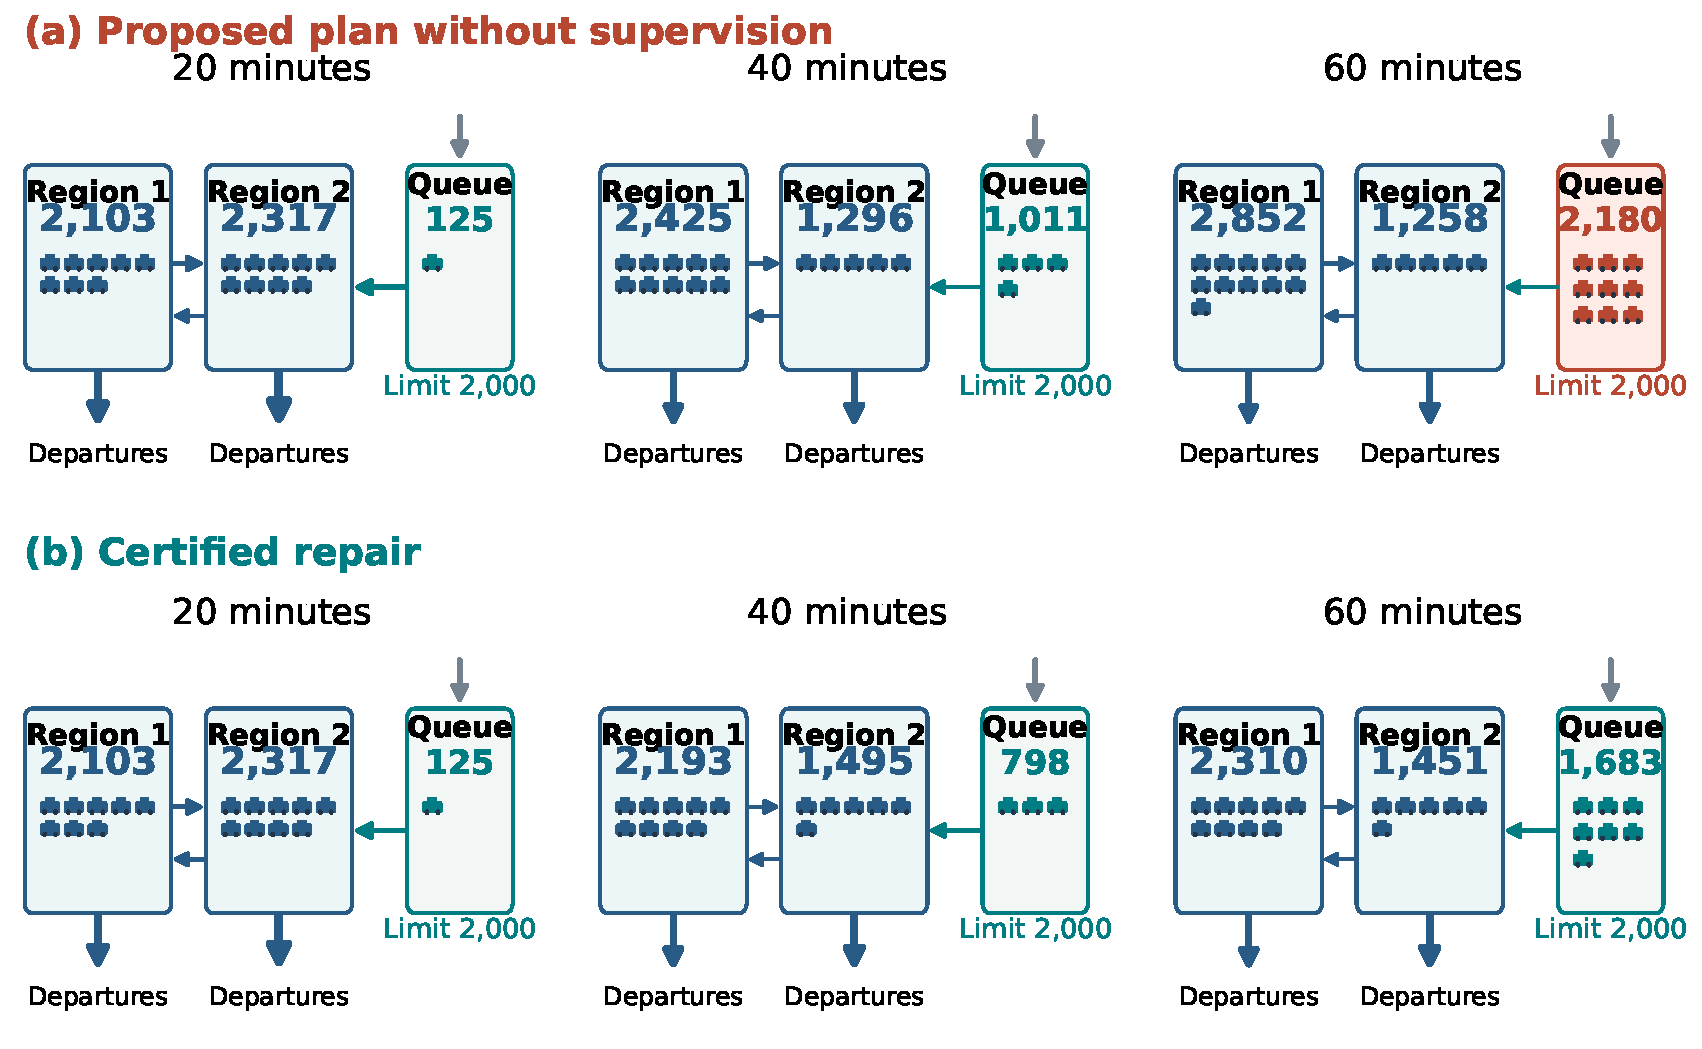
\includegraphics[width=\textwidth]{figures/supervisory_snapshots.pdf}
\caption{Traffic snapshots for the queue--deadline conflict case under the same
all-high initial state and $+300$~veh/h arrival error. Numbers are simulated
vehicle counts rounded to whole vehicles. Each car icon represents
approximately 250 vehicles, with the icon count rounded to the nearest
integer. Arrows show interregional transfers, queue admission, exterior
arrivals, and departures from the modeled network; thicker arrows indicate
larger instantaneous rates on a common scale. Departures combine local
trip completion and, for Region~2, exterior exits. Internal demand remains
in the simulation but is omitted from the drawing. Red marks a queue
above its 2000-vehicle capacity. Icon positions are illustrative.}
\label{fig:traffic-snapshots}
\end{figure}

Figures~\ref{fig:traffic-snapshots} and \ref{fig:supervisory-counts}
show how repair changes transfers, admissions and accumulations. The
unchecked proposal reaches a queue of 2180 vehicles and ends at 2852.2
vehicles in Region~1, violating both requirements. Repair at
$\lambda_{\rm rep}=0.25$ raises minute-25 admission from approximately
4594 to 5447~veh/h and $u_{12}$ from 0.397 to 0.548. Its certificate
covers the full uncertainty family through minute 60, with a continuous
queue bound of 1682.7 vehicles. The current plan also passes, allowing
the cost of the requested priority to be measured against retention.

\begin{figure}[!t]
\centering
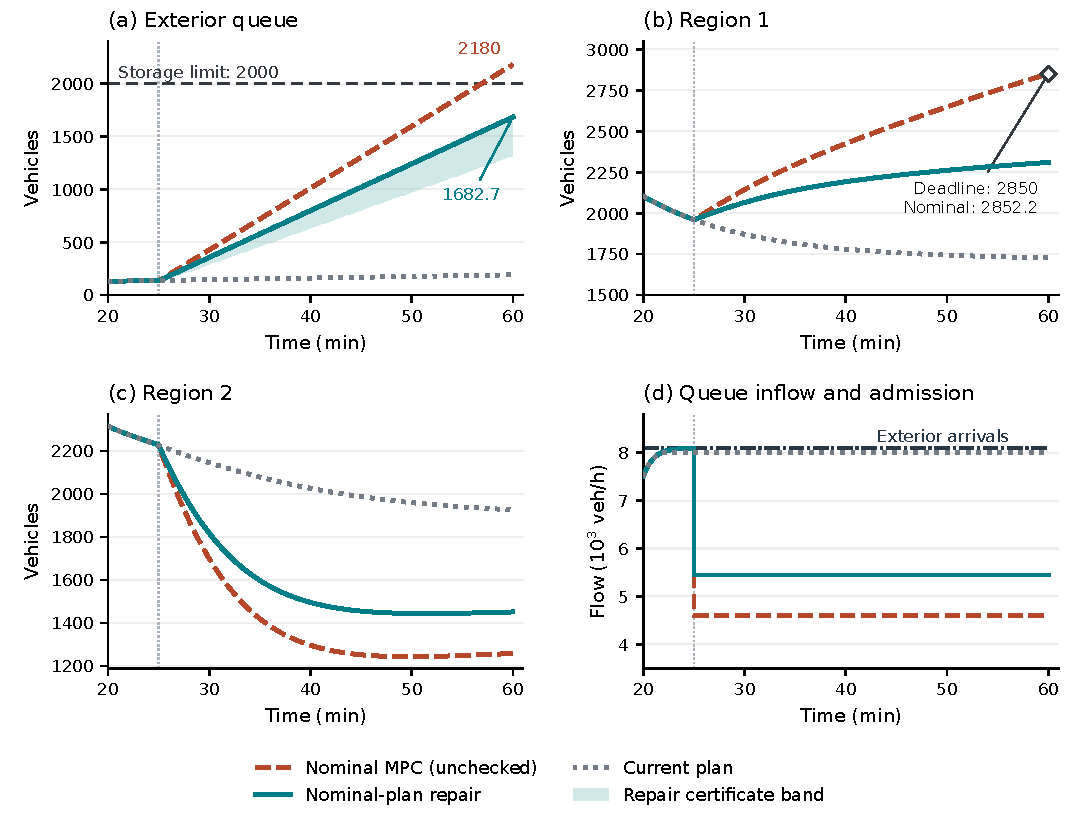
\includegraphics[width=\textwidth]{figures/supervisory_combined.pdf}
\caption{Queue--deadline conflict case with matched initial states and
arrivals: (a) exterior queue $z$, (b) Region~1 accumulation $n_1$,
(c) Region~2 accumulation $n_2$, and (d) exterior arrivals $\Lambda$ and
admission $a$ in thousands of veh/h. The dotted line marks the minute-25
input change. The horizontal line is the 2000-vehicle queue limit, and the
endpoint marker is the 2850-vehicle Region-1 requirement at minute 60.
The shaded band is the repaired plan's certified queue enclosure, whose
upper bound reaches 1682.7 vehicles.}
\label{fig:supervisory-counts}
\label{fig:supervisory-flows}
\label{fig:certified-queue-bound}
\end{figure}

Table~\ref{tab:benchmark-conflict} shows that repair lowers the priority
cost relative to retention while increasing TTS. The control-barrier-function
quadratic program (CBF-QP) protects storage but misses the deadline.
Full-scenario MPC passes this realization while its full-family check
remains inconclusive. Adaptive integration independently confirms the
illustrated trajectories and their conservation balances.

\begin{table}[!htbp]
\centering\small
\caption{Matched queue--deadline realization, minutes 20--60. TTS and
the Region-2-weighted cost $J_D$ ($p=4$) are in veh-h. Peak queue and
deadline accumulation $n_1(E)$ are in vehicles, with limits 2000 and
2850. Cert. denotes full-family certification: Yes, No (inconclusive or
violating), or a dash for not assessed. Values are rounded except the
repaired peak queue. MPC is model predictive control; CBF-QP is the
control-barrier-function quadratic program.}
\label{tab:benchmark-conflict}
\begin{tabularx}{\linewidth}{@{}Xrrrrc@{}}
\toprule
Plan & TTS & $J_D$ & Peak queue & $n_1(E)$ & Cert.\\
\midrule
Nominal MPC & 3300 & 6328 & 2180 & 2852 & No\\
CBF-QP & 3295 & 6376 & 1844 & 2917 & ---\\
Current plan & 2695 & 6814 & 194 & 1727 & Yes\\
Nominal-plan repair & 3097 & 6427 & 1682.7 & 2310 & Yes\\
Full-scenario MPC & 3267 & 6357 & 1999 & 2848 & No\\
\bottomrule
\end{tabularx}
\end{table}

\subsection{Recovery from congested conditions}
\label{sec:congested-results}
Both regions now start above critical accumulation, from the estimated
state $(4500,4500,2250,2250,750,750,500)$ vehicles. Arrivals rise from
6000 to 7800~veh/h during minutes 15--20 and remain there through minute
60. Inputs are constant over minutes 0--5 and 5--60, with a Region-1
deadline limit of 3300 vehicles. The uncertainty is
$d_x=(25,25,25,25,25,25,10)^\top$ vehicles and $\bar w=300$~veh/h.
The model and physical limits are unchanged.

The proposal minimizes the nominal priority cost with $p=4$.
A balanced-objective backup is planned from the upper uncertainty corner
and arrivals 300~veh/h above forecast, using queue/deadline planning
clearances of 1600/3000 vehicles. Certification retains the actual
2000/3300 limits. Planning and checking finish before execution.
Destination coordinates with four sub-boxes certify the backup and a
repair at $\lambda_{\rm rep}=0.35$, verifying capacity-limited admission
on every interval. All earlier grid weights violate storage for an
allowed condition: $a\le\kappa_{02}u_{02}$ gives
\[
z(1)\ge z(0)+\int_0^1\Lambda(t)\,dt
             -\kappa_{02}\int_0^1u_{02}(t)\,dt.
\]
For the upper initial queue and error $+300$~veh/h, this lower bound
exceeds 2000 vehicles at each earlier weight, including the proposal,
using exact arithmetic on the implemented coefficients.

\begin{figure}[!t]
\centering
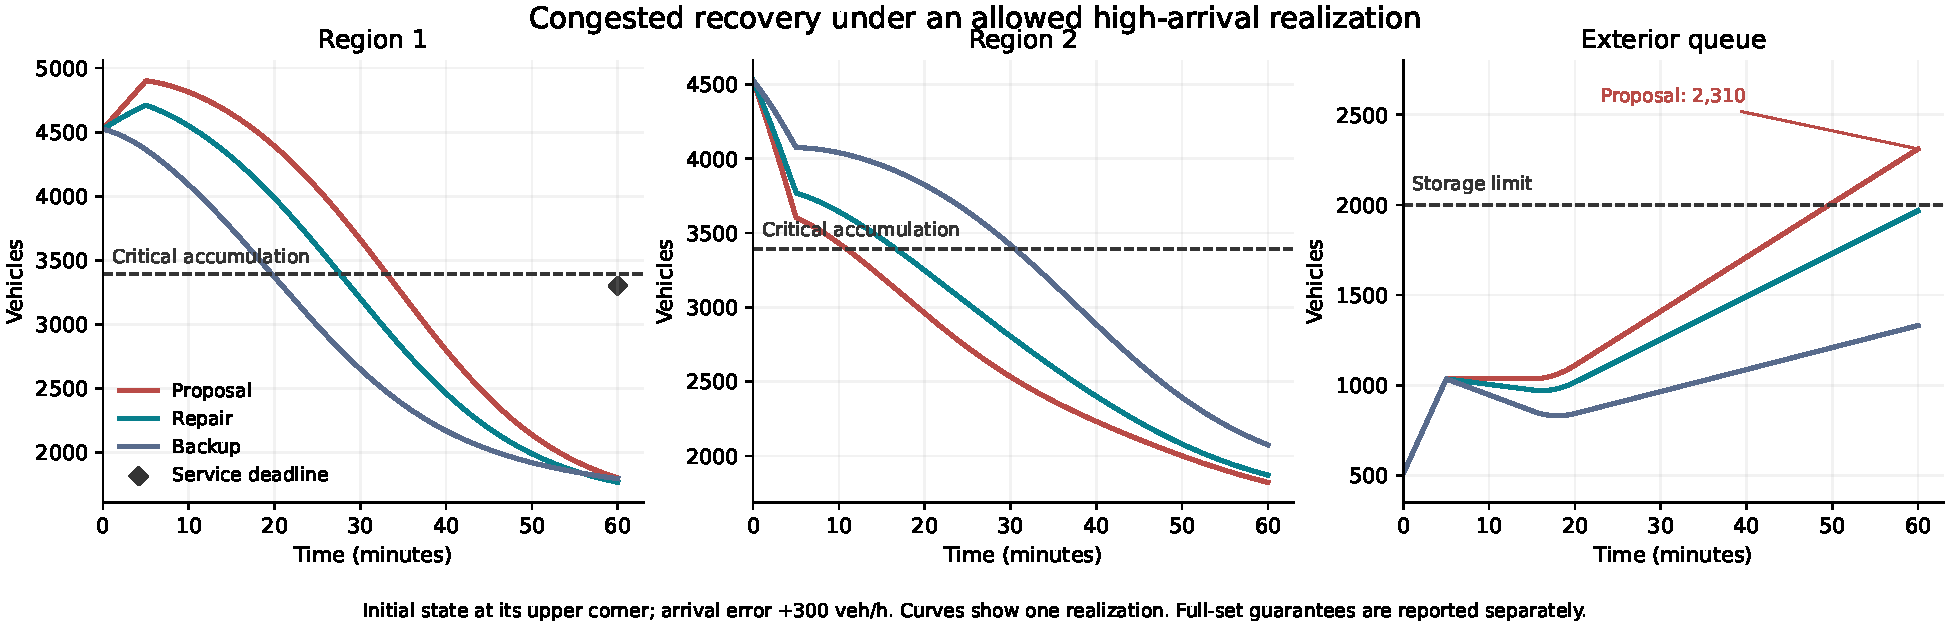
\includegraphics[width=\textwidth]{figures/wide_uncertainty_recovery.pdf}
\caption{Congested recovery for the proposed plan, the certified repair and
the certified backup. The displayed realization uses the upper initial
state corner and arrival error $+300$~veh/h. Dashed lines mark the
3391.93-vehicle critical accumulation and the 2000-vehicle queue capacity;
the diamond marks the 3300-vehicle Region-1 limit at minute 60.
Curves are simulated realizations,
while the guarantees in the text cover the full uncertainty family.
The proposed trajectory continues after overflow to show the consequence
of unchecked execution; spatial spillback is not modeled.}
\label{fig:congested-counts}
\end{figure}

The repair's certified queue maximum is below 1968 vehicles, with
minute-60 regional bounds of 2119 and 2320 vehicles, rounded upward.
The backup bounds are 1331, 2170 and 2675, respectively. Thus both plans
finish below critical accumulation throughout the specified uncertainty
family. The Region-1 requirement has substantial slack (2119 versus 3300).
Table~\ref{tab:congested-results} reports the matched-simulation costs:
relative to backup, repair reduces median priority cost by 6.05\%, raises
median TTS by 3.12\%, and recovers 78.74\% of the proposed priority benefit.

\begin{table}[!htbp]
\centering\small
\caption{Congested-start comparison over 60 minutes with regional state
error bounds of 25 vehicles, queue error 10 vehicles and arrival error
300~veh/h. Maximum queue is the largest value in 640 matched simulations;
physical and service passes count simulations satisfying those constraints.
TTS is total time spent in both regions and the queue. $J_D$ is the
Region-2-weighted cost with $p=4$; both costs are medians in vehicle-hours.
Certificates cover the full uncertainty family.}
\label{tab:congested-results}
\begin{tabularx}{\linewidth}{@{}Xrrr@{}}
\toprule
Measure & Proposed & Repaired & Backup\\
\midrule
Maximum simulated queue (vehicles) & 2310.0 & 1967.2 & 1330.7\\
Physical passes & 320/640 & 640/640 & 640/640\\
Service passes & 640/640 & 640/640 & 640/640\\
Median TTS (vehicle-hours) & 7488.3 & 7229.7 & 7011.1\\
Median $J_D$ (vehicle-hours) & 15499.7 & 15773.9 & 16789.5\\
Full-hour certificate & Rejected & Passed & Passed\\
\bottomrule
\end{tabularx}
\end{table}

The coordinate choice matters: an unsplit conservation check certifies
28.5 minutes, unsplit destination coordinates reach 54 minutes, and
destination coordinates with subdivision certify the hour and deadline.
The failing conservation-bound remainder is dominated by arrival forcing
(58.63\%) and Jacobian/generator mismatch (41.15\%), with a 0.22\%
predictor-defect contribution. Detailed diagnostics are in the reproduction
materials. Regional terminal widths remain about 12--27 times the sampled
spreads, while certified and sampled queue widths both equal 620 vehicles
to numerical precision: 20 from the initial queue range and 600 from
arrival error. Samples do not establish the full reachable set. The
regional initial bound is 0.56\% of 4500 vehicles, where fitted outflow
is 7.05\% below capacity.

Keeping the plans, destination proportions, initial queue, uncertainty
and deadline fixed, we test equal regional totals of 3500, 4000, 4500,
5000, 5500, 6000, 6500, 7000, 8000 and 9000 vehicles. The portfolio
certifies both plans at the first three levels: unsplit destination
coordinates pass at 3500/4000, and four boxes are needed at 4500.
No higher tested level passes. At 5000, the upper-corner high-arrival
simulation leaves the backup's Region~2 at 3520 vehicles, above critical
accumulation, and the repair ends with 6596 vehicles in Region~1, missing
its deadline. These outcomes concern the fixed plans, not an upper limit
on recovery with redesigned control. At 4500, portfolio verification
takes 82.6 seconds for backup and 82.3 for repair, including the two
unsuccessful unsplit checks and four passing sub-boxes.

\subsection{Certification and repair across operating conditions}
\label{sec:structure-results}
\label{sec:structure-online}
\label{sec:uncertainty-results}
We next compare the bound constructions of
Section~\ref{sec:structure-certificate}, holding a two-block MPC plan fixed
over minutes 0--60. The arrival-error bound is 60~veh/h, the Region-1
deadline is 2850 vehicles, and
$d_x=(d,d,d,d,d,d,\min(d,10))^\top$ for
$d\in\{1,5,10,25,50,100\}$ vehicles.

\begin{figure}[!t]
\centering
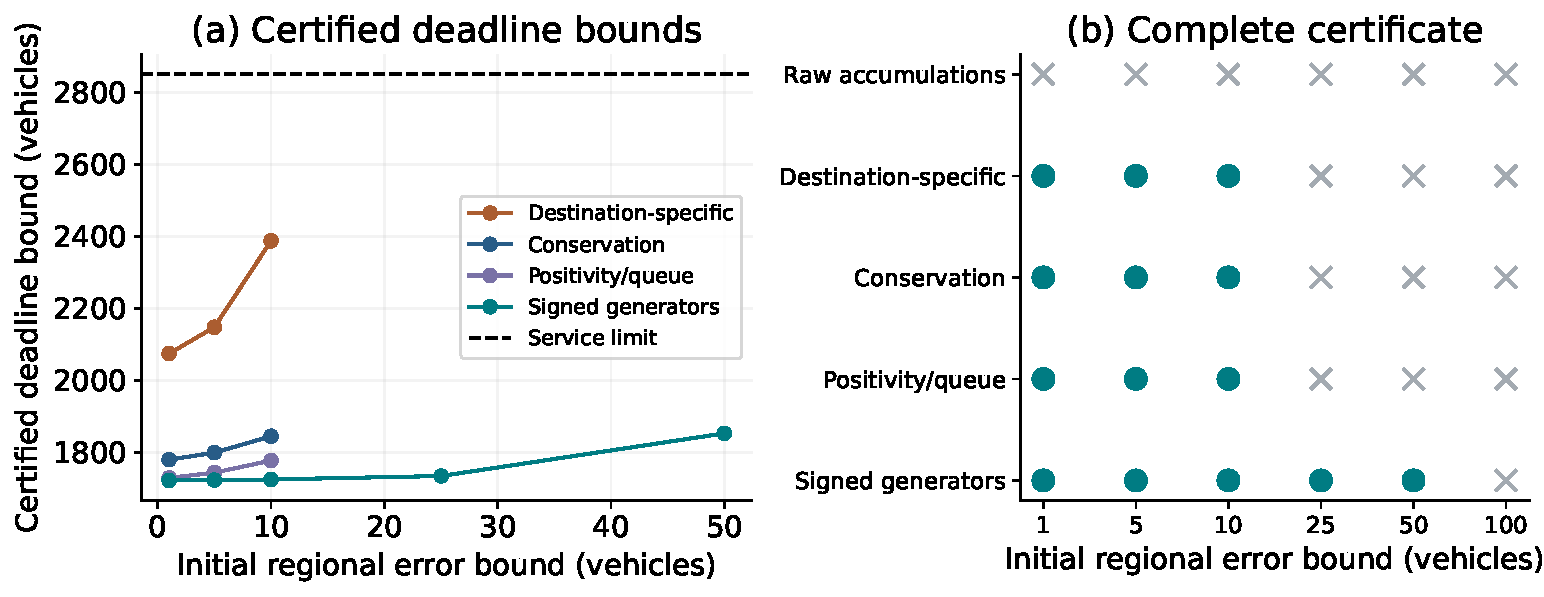
\includegraphics[width=\textwidth]{figures/structure_certification_comparison.pdf}
\caption{Effect of traffic structure for the fixed-plan experiment.
(a) Region-1 deadline bounds for complete passing certificates, with
the 2850-vehicle service limit marked. Lines connect tested settings only.
(b) Every tested initial regional error bound: circles indicate a complete
certificate and crosses an inconclusive check. Queue uncertainty is
capped at 10 vehicles, and the arrival-error bound is 60~veh/h.
No deadline value is plotted when an earlier physical check prevents
completion. Destination-specific denotes coordinates for the separate
destination accumulations; conservation adds their allocated queue shares.}
\label{fig:structure-comparison}
\end{figure}

Figure~\ref{fig:structure-comparison} shows that signed propagation
passes through $d=50$, compared with $d=10$ for the interval methods.
At $d=1$, adding queue shares reduces the destination-coordinate deadline
bound from 2075 to 1780 vehicles; signed propagation gives 1722.
The portfolio retains the signed conservation result through $d=50$
and adds no pass at $d=100$. This sweep keeps queue error at most ten
vehicles. At arrival error 300~veh/h and $d=1$, positivity/queue bounds
are tighter than signed bounds (2009 versus 2256 vehicles); at $d=25$,
only the signed method passes, with a 2504-vehicle bound. Together with
the opposite coordinate ordering in the congested case, these results
support testing complementary bounds under verified traffic conditions.

The broader comparison uses 80 minute-20 contracts with the 30\%
one-hour event and $d_x=d\mathbf1_7$, including the queue.
The 72 development cases cross $d\in\{1,10,25,50\}$ vehicles,
$\bar w\in\{60,150,300\}$ veh/h, $\eta\in\{2750,2850,2950\}$ vehicles
and $p\in\{2,4\}$. Eight held-out cases use
$d\in\{5,20\}$, $\bar w\in\{100,225\}$,
$\eta\in\{2800,2900\}$ and $p=3$. Full-scenario MPC uses one-vehicle
prediction clearance with settings fixed across both sets.

\begin{table}[!htbp]
\centering\small
\caption{Availability across 80 contracts. Baseline denotes unsplit signed
conservation checks; Portfolio is the fixed four-member procedure.
Simulation passes require all 640 realizations in a contract to satisfy
physical and service requirements. Proposal rows evaluate all 80 candidates;
repair rows evaluate only selected outputs, giving denominators 74 or 80.
Certified availability always uses the full 80-contract denominator.
MPC is model predictive control. Portfolio rechecking leaves plans unchanged;
repair rows report the baseline search.}
\label{tab:benchmark-deadlines}
\label{tab:fixed-portfolio}
\begin{tabularx}{\linewidth}{@{}Xlrr@{}}
\toprule
Planning/execution option & Check & \shortstack{Simulation\\passes} & \shortstack{Certified\\availability}\\
\midrule
Nominal MPC & Baseline & 36/80 & 36/80\\
Five-scenario MPC & Baseline & 40/80 & 40/80\\
Full-scenario MPC & Baseline & 80/80 & 44/80\\
Full-scenario MPC & Portfolio & 80/80 & 50/80\\
Nominal MPC with repair & Baseline & 74/74 & 74/80\\
Full-scenario MPC with repair & Baseline & 74/74 & 74/80\\
Repair with new backup & Baseline & 80/80 & 80/80\\
\bottomrule
\end{tabularx}
\end{table}

The portfolio retains all baseline passes, adds six full-scenario
certificates through unsplit destination coordinates, and leaves nominal
availability at 36/80. The six additions are development cases; held-out
outcomes are unchanged, and subdivision adds no further passes.
Median portfolio verification times are 40.1 seconds for nominal and
10.7 for full-scenario proposals (ranges 9.3--89.7 and 9.7--72.7).
These include unsuccessful attempts under the workload described above.

In the baseline repair study, the remaining current plan passes its new
backup check in 68/80 contracts. Selecting 36 nominal proposals and 38
repairs gives 74 certified outputs. Newly constructed backups pass in
the twelve cases where the remaining plan fails its new check; six already
have passing proposals, and the other six gain outputs, giving 80/80.
This illustrates the same-contract backup condition in
Lemma~\ref{thm:repair-grid}. Nine nominal proposals pass with $d=50$
without a separate queue cap. The uncertainty breakdown is in
\appref{app:additional-numerics}.

Nominal proposals violate storage in 44 contracts and the deadline in
36, with median maximum excesses of 90.3 and 19.4 vehicles, respectively.
These observed violations differ from inconclusive checks. In a separate
one-adverse-realization-per-contract comparison, the CBF-QP satisfies
physical constraints in all 80 runs and service deadlines in 44.

For matched realization $\omega=(x_0,w)$, define the repair's priority
improvement, TTS change and recovered benefit relative to backup $P^B$
and proposal $P^0$ by
\begin{equation}
\begin{aligned}
\Delta J_\omega&=100\frac{J_D(P^B;\omega)-J_D(P^R;\omega)}{J_D(P^B;\omega)},\\
\Delta D_\omega&=100\frac{J_Q(P^R;\omega)-J_Q(P^B;\omega)}{J_Q(P^B;\omega)},\\
B_\omega&=\frac{J_D(P^B;\omega)-J_D(P^R;\omega)}{J_D(P^B;\omega)-J_D(P^0;\omega)}.
\end{aligned}
\label{eq:benchmark-repair-metrics}
\end{equation}
Here $P^R$ is the selected repair and $J(P;\omega)$ is its realized cost.
Across 24,320 realizations from the 38 repaired contracts, the medians
of $\Delta J_\omega$, $\Delta D_\omega$ and $100B_\omega$ are 5.7\%,
16.1\% and 91.7\%, with interquartile ranges 3.9--6.2\%, 8.8--19.6\%
and 78.2--95.9\%. All benefit denominators are positive. These describe
the pooled test realizations, not confidence intervals; the complete
distributions are in the reproduction materials.

\paragraph{Several-region examples}
\label{sec:network-transfer-results}
The extension in Section~\ref{sec:network-extension} is evaluated under
the fixed routing and allocation in \appref{app:network-transfer}:
the conservation construction certifies two- and three-region rings
with an entry queue per region (six and twelve states). At regional
error $d=25$ vehicles, the two-region plan passes with arrival error
300~veh/h per queue and the three-region plan with 60~veh/h. Their
largest certified deadline bounds are 1552 and 2060 vehicles against
a 2700-vehicle limit. Destination coordinates alone leave both checks
inconclusive. Successful twelve-state checks take 5.20--5.28 seconds
for 120 intervals; the complete sixteen-attempt sweep is retained with
the reproduction records.

\subsection{Successive requests and computation delays}
\label{sec:sequential-handover-results}
We now test the replacement and delayed-activation rules of
Sections~\ref{sec:new-execution} and \ref{sec:planned-handover}.
A certified $p=4$ repair begins at minute 20. Requests at minutes 25
and 30 propose the remaining $p=2$ full-scenario and $p=4$ nominal plans,
respectively. Each is checked from a containing reachable-state box,
with unchanged physical limits and a minute-60 deadline. These stored
requests isolate supervision from language interpretation.

For $(d,\bar w,\eta)=(1,60,2850)$ both replacements pass; for
$(1,300,2850)$ the first passes and the second is inconclusive; for
$(50,60,2950)$ both are inconclusive. All sampled unchecked schedules
in these three preselected cases satisfy the constraints. In the wide-set
case, propagated boxes include inadmissible combinations without proving
that an actual state reaches them. Retention therefore preserves the
current certificate even when a new check fails.

The tight-deadline case $(1,300,2750)$ in
Figure~\ref{fig:successive-traffic} comes from a scan of 36 matched
development-contract pairs, thirty of which support the initialized
sequence. Three unchecked sequences overflow, by 5.59, 9.62 and 17.60
vehicles. The figure shows the first such case: the supervisor accepts
the minute-25 replacement and rejects the minute-30 proposal.
Unchecked execution reaches 2005.59 vehicles, confirmed by adaptive
integration, and passes only 512/640 simulations. Supervised execution
passes 640/640. Its median TTS is 8.2\% below retaining the initial plan,
with a 5.2\% greater median time-varying-priority cost than unchecked switching.

\begin{figure}[!t]
\centering
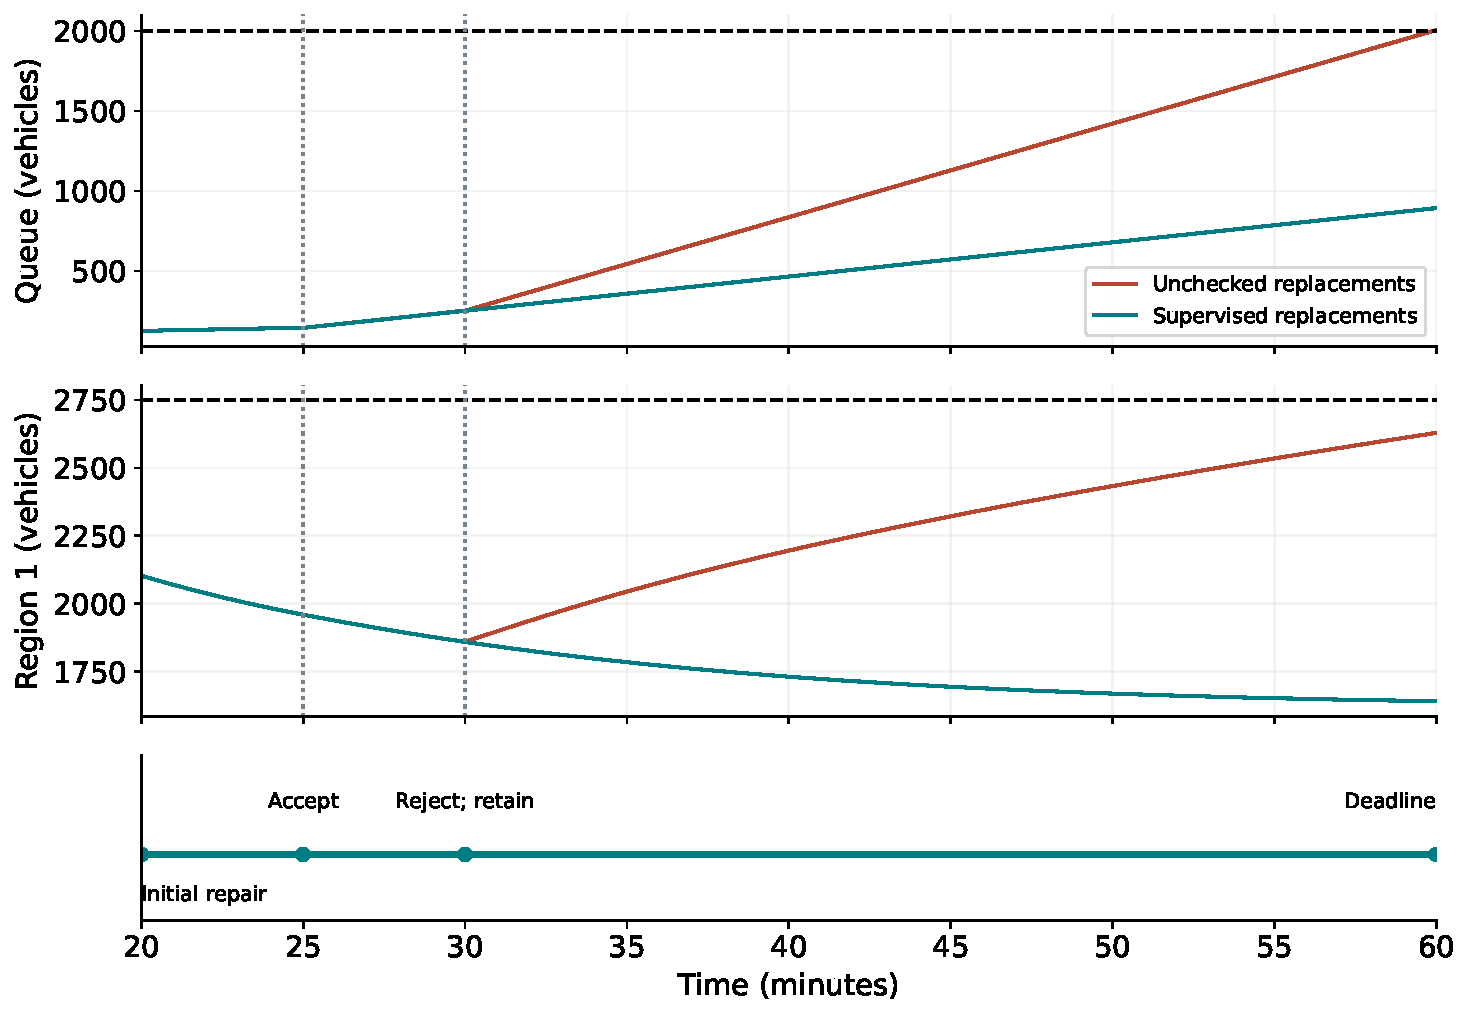
\includegraphics[width=\textwidth]{figures/successive_decisions_traffic.pdf}
\caption{Successive requests in the tight-deadline case, with the same
all-high initial corner and constant $+300$~veh/h arrival error for both
executions. The upper panels show exterior waiting and Region-1
accumulation. Dashed horizontal lines mark the 2000-vehicle queue
capacity and 2750-vehicle service limit at minute 60. Vertical dotted
lines identify requests at minutes 25 and 30. The lower timeline gives
the supervisory decisions. The unchecked schedule activates both
proposals; the supervised schedule retains the minute-25 replacement
after rejecting the minute-30 proposal.}
\label{fig:successive-traffic}
\end{figure}

\paragraph{Delayed activation}
\label{sec:delayed-handover-results}
Seventeen contracts are checked with one-, two- and five-minute activation
delays while the current plan continues. Propagation supplies the future
state set and deadlines remain fixed. Timely replacements number 8/17,
11/17 and 11/17, respectively, with 9/17, 6/17 and 6/17 retentions.
All $51\times640=32{,}640$ simulations satisfy physical and service
requirements. Three one-minute results arrive late. A longer delay
allows more computation but changes the activation set and leaves less
time before the deadline. The study records propagation, planning and
checking time. Separately measured baseline medians are 8.1 seconds for
one proposal check, 52.7 for proposal plus repair checks through
$\lambda_{\rm rep}=0.25$, and 63.4 including backup rechecking, excluding
planning. Detailed timings are in \appref{app:additional-numerics}.

\subsection{Agent interpretation and certified execution}
\label{sec:task-state-live}
\label{sec:queue-live-pilot}
\label{sec:primary-memory-pressure}
Finally, we evaluate instruction interpretation within the planning interface
of Section~\ref{sec:agent-requests}. The agent study uses
\texttt{gpt-5.4-mini-2026-03-17}, with reasoning
disabled and strict function schemas. Eight traces pair four operator
histories across the history-only and task-record formats under corrupted
memory. Each trace uses the agent's chosen objective in a fresh MPC solve;
the tool interface forwards the proposal directly to the supervisor.
After rejection, repair is attempted only if the agent requests it and
is checked before execution. The study contains thirteen live calls and
640 simulations per executed schedule.

\begin{table}[!htbp]
\centering\small
\caption{Agent planning under corrupted memory, with four histories per
format. History only supplies instructions and interaction history; Task
record additionally supplies the current priority and timing. Objective
correct counts traces matching the operator's priority. Repairs executed
counts traces activating a checked repair. Feasible trajectories satisfy
physical and service requirements across $4\times640=2560$ simulations
per format.}
\label{tab:benchmark-api-execution}
\begin{tabularx}{\linewidth}{@{}Xrrr@{}}
\toprule
Format & \shortstack{Objective\\correct} & \shortstack{Repairs\\executed} & \shortstack{Feasible\\trajectories}\\
\midrule
History only & 1/4 & 1/4 & 2560/2560\\
Task record & 4/4 & 4/4 & 2560/2560\\
\bottomrule
\end{tabularx}
\end{table}

In three history-only traces, a certified MPC plan pursues the wrong
regional objective. The task record improves objective selection in
these examples, while the supervisor independently enforces physical
and service requirements (Corollary~\ref{cor:agent-independent-execution}).
A separate 96-call interpretation pilot uses stored plans: task records
give 24/24 correct objectives with both clean and corrupted memory,
compared with 19/24 and 15/24 for history alone. Its full scoring breakdown
is retained with the reproduction materials; its design is in
\appref{app:additional-numerics}. These studies cover one model version
and a small set of histories, not every task-record operation.

\section{Operational Insights and Implementation}
\label{sec:new-discussion}
\label{sec:information-model-scope}

The experiments distinguish the traffic performance of a proposed plan
from the guarantee available before execution. Full-scenario MPC satisfies
every tested simulation in all 80 contracts. The conservation-coordinate
check certifies 44 proposals over the full uncertainty family, and the
fixed portfolio raises this count to 50. A failed check can
therefore leave a useful plan undecided. Tighter traffic-state bounds and
checked repair provide two ways to obtain an executable alternative.
In the 38 original repair cases, repair recovers a median 91.7\% of the
requested benefit at a median 16.1\% increase in TTS relative to the
current plan. This tradeoff makes the traffic cost of pursuing a regional
priority explicit.

Computation and traffic evolution must be considered together. The
delayed-activation study accepts 8, 11 and 11 of 17 replacements with
one-, two- and five-minute delays. Additional computation time can help,
but the system also moves before activation. Certification alone takes
approximately a minute in the illustrated repair case, excluding planning,
and observed runtimes depend on hardware and load. Implementations need a
certified initial plan, matching model and task versions, and enough time
for propagation, planning, checking and actuation. In the small agent
study, the task record improves objective selection while the supervisor
checks physical and service requirements independently of that selection.

The numerical scope is limited to a literature MFD, synthetic internal
demands, known event means, and the same dynamics for simulation and
certification. The results cover the specified state and arrival errors,
not unmodeled changes in production, routing, internal demand, release
rate or entrance capacity. The one-vehicle cases assume tightly known
initial conditions. Wider bounds and queue caps vary by study as stated
in Section~\ref{sec:experimental-setup}; they require field calibration.
The congested-start experiment certifies full-hour recovery with regional
state errors of 25 vehicles, queue error 10 vehicles and arrival error
300~veh/h, using destination-specific coordinates and four initial boxes.
The fixed-plan sweep retains certified recovery through the tested
4500-vehicle starting point. Its capacity-limited branch, slack service
deadline and remaining regional enclosure conservatism delimit the evidence. The connected-ring studies use their own fixed routing and
allocation assumptions.

Regional totals do not determine destination mixtures, so deployment
requires a joint estimate set for destination-specific accumulations and queues,
including measurement bias and timing errors. Destination decomposition
is also treated as uncertain in robust perimeter control
\cite{haddad2015robust}. Additional model error, or feedback using estimated
states, requires validated bounds on its effect during execution. A fresh
estimate set disjoint from the current certificate's reachable set signals
inconsistent assumptions; the present guarantee does not specify recovery
from that condition. Continuation beyond a finite plan additionally needs
the invariant policy, terminal-set inclusion and service coverage in
\appref{sec:terminal-backup}, with sustained arrivals compatible with
storage and discharge.

\section{Conclusions}
\label{sec:new-conclusion}

This paper develops a dual-agent framework in which an AI agent proposes
urban perimeter-control plans and a rule-based supervisory agent checks
them before execution. Under the stated traffic and interface assumptions,
the framework verifies physical constraints and service requirements for
every activation state and arrival allowed by the supplied bounds. The useful coordinate choice depends on verified admission structure:
conservation coordinates cancel shared admission, while destination-specific
coordinates retain regional independence from arrival error under
capacity-limited constant inputs. Subdividing the initial set can further
reduce overestimation. Across the 80 contracts, the fixed portfolio certifies 36 nominal and
50 full-scenario proposals, including six additional full-scenario plans
accepted without modification. The baseline repair studies raise nominal
plan availability from 36 to 74, and to 80 with newly certified backups. Rejected or late replacements leave the current plan
under its existing guarantee, and additional terminal conditions support
operation beyond the planned period. The congested experiment certifies recovery with 25-vehicle regional
state errors, 10-vehicle queue error and 300~veh/h arrival error.
Separate experiments illustrate supervisory decisions under successive
requests, computation delays and agent-context errors, while several-queue
examples extend the construction. Their scope is limited
to the stated model and uncertainty sets.

Future work will develop joint estimates of regional destination-specific accumulations
and queues, calibrate their uncertainty bounds, and account for estimation
errors in feedback execution. Further studies will address discrepancies
between the model and observed traffic, broaden congested-operation
tests to larger uncertainty sets and repeated estimation updates, and
evaluate larger sets of agent models and operator histories. Another
direction is to choose activation times jointly with the plan, accounting
for sensing, computation, actuation and pending service deadlines.

\section*{CRediT authorship contribution statement}
\textbf{Ali Eslami:} Conceptualization, Methodology, Software, Validation,
Formal analysis, Investigation, Data curation, Visualization,
Writing and editing.
\textbf{Jiangbo Yu:} Supervision, Review and editing.

\section*{Declaration of competing interests}
The authors declare that they have no known competing financial interests or
personal relationships that could have appeared to influence the work
reported in this paper.

\section*{Data and code availability}
Reproducibility materials include the traffic models, planning and
certification implementations, experiment protocols, stored agent requests
and responses, certificate records, and simulation outputs described in the
experimental settings in \appref{app:experimental-settings}. The materials are maintained at
\url{https://github.com/AlienEslami/agentic-perimeter-runtime-certification}.


\appendix
% Use appendix letters for equations while retaining full appendix section titles.
\renewcommand{\theequation}{\Alph{section}.\arabic{equation}}
\numberwithin{table}{section}
\renewcommand{\thetable}{\Alph{section}.\arabic{table}}
\Needspace{0.78\textheight}
\section{Notation}
\label{app:notation}

\begingroup
\fontsize{9}{10}\selectfont
\renewcommand{\arraystretch}{0.98}
\setlength{\LTcapwidth}{\textwidth}
\begin{longtable}{@{}p{0.20\linewidth}>{\raggedright\arraybackslash}p{\dimexpr0.80\linewidth-2\tabcolsep\relax}@{}}
\caption{Notation used throughout the paper. Traffic accumulations and state bounds are in vehicles,
flow rates are in veh/h, and time is in hours unless stated otherwise.}
\label{tab:nomenclature}\\
\toprule
Symbol & Meaning\\
\midrule
\endfirsthead
\multicolumn{2}{@{}l@{}}{Table~\thetable\ (continued)}\\
\toprule
Symbol & Meaning\\
\midrule
\endhead
\midrule
\endfoot
\bottomrule
\endlastfoot
$n_i$, $n_{ij}$ & Regional accumulation; vehicles in region $i$ destined for $j$\\
$z$, $x$, $M$, $M_P$ & Exterior queue; traffic state; total accumulation; its trajectory under plan $P$\\
$\widehat x_{t_0}$, $\mathcal I_{t_0}$ & Supplied state estimate and containing state set at plan activation\\
$u_{ij}$, $a$ & Perimeter control input; realized exterior admission flow\\
$N$, $n_{\rm acc}$, $n_q$ & Numbers of regions, destination-specific accumulations, and entry queues\\
$\mathcal L_i$, $\ell_i$ & Total lane length (lane-km); mean distance traveled within region $i$ (km)\\
$\rho_i$, $V_i(\rho_i)$ & Regional density (vehicles per lane-km); average speed (km/h)\\
$n_i^{\rm crit}$ & Critical accumulation at a capacity maximum of the regional MFD\\
$G_i$, $m_{ij}$ & Regional MFD outflow; destination-specific potential outflow (veh/h)\\
$v_i(n)$, $v(n)$ & Regional per-vehicle outflow rate $G_i(n)/n$ (h$^{-1}$); common fitted rate in the two-region experiments\\
$x_{\rm net}$, $f_{\rm net}$, $B_w$ & Network state, nominal dynamics, and arrival-error incidence matrix\\
$B(u)$, $m(c)$ & Routing and control matrix; vector of potential outflows\\
$\pi$, $\tau_q$, $\kappa_{02}$ & Region-1 entry fraction; queue-release time; admission capacity\\
$n_i^{\max}$, $z^{\max}$ & Regional operational accumulation limit; exterior storage capacity\\
$\delta_1^u$, $\delta_2^u$ & Allowed differences between paired perimeter control inputs\\
$\Lambda$, $\widehat\Lambda$, $w$ & Exterior arrival rate, forecast, and forecast error\\
$d^{\rm int}_{ij}$ & Internal demand in region $i$ for destination $j$ (veh/h)\\
$d_x$, $d_x(t_i)$, $d$ & Initial state-error bounds, bounds at $t_i$, and scalar sweep parameter\\
$\bar w$ & Arrival-forecast error bound (veh/h)\\
$\mathcal S_t$, $\mathcal S_t^{\rm rep}$ & Full decision record and its repair fields\\
$\mathcal H_t$, $\mathsf{ver}_t$ & Current certificate; identifier of model, forecast and constraint versions\\
$\mathcal O_t$, $\mathcal W_t$ & Pending service requirements; allowed arrival-error family\\
$P$, $P_i^0$, $P_i^{\rm cand}$ & Generic plan, original proposal, and candidate (original or repaired)\\
$P_t^{\rm cur}$, $E_{\rm cur}$ & Current executing plan and its original expiry\\
$P^B$, $E_B$, $\mu_{\rm term}$ & Repair backup, its expiry, and terminal policy beyond expiry\\
$t_i^{\rm req}$, $t_i$, $t_{\rm ready}$ & Request, decision/activation, and certificate-completion times\\
$T^{\rm prio}$, $E$ & Priority expiry; plan expiry\\
$\mathsf{Comp}$, $q_i^A$ & Request compiler; validated planning request ($\bot$ if invalid)\\
$P_a$, $c$ & Admission-allocation matrix; vector of destination-specific accumulations\\
$\gamma_q^{\rm rel}$, $u_q^{\rm in}$ & Queue-$q$ release rate (h$^{-1}$) and entrance input\\
$u_i^{\rm ring}$ & Perimeter input from region $i$ to the next region in a directed ring\\
$\eta$ & Regional-priority task's Region-1 accumulation limit (vehicles)\\
$T_r$, $g_r$, $\eta_r$ & Service deadline, constraint coefficients and limit\\
$\theta_i$, $\lambda_{\rm rep}$ & Agent task record; predictive-repair interpolation weight\\
$K_b$, $N_b$, $\mathcal K$ & Feedback gain; control-block count; terminal invariant set\\
$N_{\rm dec}$ & Number of subsequent decision times in the finite replacement theorem\\
$\beta_j^{\rm phys}$, $b_a$ & Physical constraint limit; vehicle-admission incidence vector\\
$y$, $L$ & Transformed state and its fixed invertible coordinate map\\
$\mathsf R_{ik}^{(j)}$ & Fixed share of destination-$j$ flow routed from $i$ to $k$\\
$\mathsf k$, $N_{\rm box}(\mathsf k)$ & Verification-configuration index and number of initial cover members\\
$\mathcal R_P(t)$ & Union of certified reachable enclosures at time $t$\\

$r_l$, $R_l$ & Initial error bounds and trial error bounds on interval $l$\\
$r^{\rm gen}$, $r^\zeta$ & Continuous bounds on signed-generator and remainder contributions\\
$a_{il}^{\rm cmp}$, $b_{ijl}^{\rm cmp}$, $c_{il}^{\rm cmp}$ & Diagonal, off-diagonal, and forcing bounds in componentwise comparison\\
$r_l^{\rm rem}$ & Initial bound on the remainder $|\zeta_l(0)|$ on interval $l$\\
$A_l^{\rm mv}$, $A_l^0$ & Mean-value Jacobian and fixed generator-propagation matrix\\
$\mathcal G_\Gamma$ & Set enclosing the generator matrices over a verification interval\\
$\xi$, $\Gamma_l$, $\zeta_l$ & Shared initial uncertainty, its coefficient matrix and error remainder\\
$z_e$, $e_i^{\rm abs}$ & Transformed prediction error; its component magnitude $|(z_e)_i|$\\
$J_Q$, $J_D$ & Total-time-spent and weighted-priority objectives\\
$p$, $\mathbf p_l$ & Regional-priority weight; state predictor\\
$\mathcal C$, $\mathcal F_{\mathcal C}$, $\widehat{\mathcal F}_{\mathcal C}$ & Planning contract; robustly feasible and certified plan sets\\
$\overline M$, $\Psi$ & Metzler comparison matrix; integral of its exponential\\
$N_{\rm T}$ & Matrix-exponential series order\\
$\mathcal V_{\rm term}$, $\overline{\mathcal V}_{\rm term}$ & Terminal Lyapunov function and its sublevel-set limit\\
$j_{\rm run}$, $j_{\rm end}$, $T_{\rm cost}$ & Running cost, terminal cost, and horizon for the repair-cost bound\\
$\omega=(x_0,w)$ & Matched initial state and arrival-error realization\\
$B_\omega$ & Fraction of requested priority benefit recovered by repair\\
$\mathrm{TTS}$ & Total time spent, including exterior waiting; vehicle-hours (veh-h)\\
\end{longtable}
\endgroup

\section{Essential Experimental Settings}
\label{app:experimental-settings}
\label{app:reusable-benchmark}
\label{sec:supp-queue-settings}
\label{app:benchmark-details}

\paragraph{Implementation coordinates}
The stored numerical implementation represents 100 vehicles as one unit.
For implementation state $\widetilde x=x/100$, physical-unit and stored
quantities satisfy
\[
\widetilde f(\widetilde x,u,t)=f(100\widetilde x,u,t)/100,\qquad
\widetilde w=w/100,\qquad
\widetilde G(\widetilde n)=G(100\widetilde n)/100.
\]
Control inputs and time are unchanged. A stored feedback law
$u=\widetilde k_b+\widetilde K_b\widetilde x$ corresponds to
$k_b=\widetilde k_b$ and $K_b=\widetilde K_b/100$ in this paper.
Stored predictors, state radii, signed generators, and additive error
bounds are multiplied by 100 to obtain their physical-unit values.
The transform $L$ is unchanged, and
$D_{\widetilde x}\widetilde f=D_x f$ at corresponding states and controls.
For a physical constraint $Hx+Ju\le\beta$, the equivalent stored form is
$100H\widetilde x+Ju\le\beta$.
A service limit $g^\top x\le\eta$ becomes
$100g^\top\widetilde x\le\eta$.
These conversions preserve the represented trajectories, control inputs,
and constraint satisfaction. Reported costs and vehicle counts already
use physical units.

\paragraph{Primary state and plans}
The network-efficiency and regional-priority tasks start at minute 20 ($t_0=1/3$ h) with the state center, in the order of
\eqref{eq:new-state}, in vehicles,
\[
\begin{aligned}
\widehat x_{t_0}=(&2102.0544601495207,2315.6747836310867,\\
&1420.9387548878382,1487.7124601919054,\\
&240.28346640030684,301.84193919155455,\\
&124.10781134202304).
\end{aligned}
\]
The current-plan comparator uses $(1,1,0.667015677,1)$ in control-input order
$(u_{12},u_{21},u_{02},u_{20})$, in five- and
35-minute blocks ending at minute 60. Its remaining schedule is rechecked for
each contract. If a new backup is needed, construction tries network TTS
followed by moderate Region-2 priority and certifies the result before
repair. The ordered repair grid is given in Section~\ref{sec:experimental-setup}.
Plans are converted to control-input coefficients and checked against exact
actuator constraints. State and service checks use 15-second verification subintervals.

\paragraph{Trajectory simulations and comparisons}
Simulations use the five arrival-error profiles in
Section~\ref{sec:experimental-setup}, paired with all 128 initial-box
corners for constant plans. The CLF comparison uses sixteen corners,
every eighth entry of the lexicographic $\{-1,+1\}^7$ list.
Simulations use fourth-order Runge--Kutta
(RK4) integration with ten-second steps, supplemented by independent
adaptive eighth-order Runge--Kutta (DOP853) integration and conservation
checks. CLF and CBF comparators use exact simulated states at ten-second
updates, with constant control inputs between updates.
The CLF extension combines regional-error correction with
linear-quadratic admission/exit feedback and reference totals
$(2700,3200)$ vehicles. The CBF-QP minimizes deviation from
MPC subject to control-barrier-function inequalities for the physical constraints, with gain $6$ h$^{-1}$
and the worst queue-arrival error \cite{ames2017}. Its service deadline
is an evaluation criterion. 

\paragraph{Future activation}
\label{supp:detail:sec:delayed-handover-results}
\label{app:sequential-handover}
The seventeen delayed-activation contracts comprise the eight extremes
$(d,\bar w,\eta,p)\in\{1,50\}\times\{60,300\}\times
\{2750,2950\}\times\{4\}$, primary $(1,300,2850,4)$ contract and eight
held-out contracts. The active plan supplies the activation box
$\mathcal I_{t_a}^+=\widehat x_{t_a}+[-d_x(t_a),d_x(t_a)]$, where
$(d_x(t_a))_i=\sum_j|(L^{-1})_{ij}|(r_{t_a})_j$, by outward conversion of its
endpoint bound that preserves shared uncertainty dependence. The recorded total computation time includes propagation,
optimization, checking and repair.

\paragraph{Connected rings}
\label{app:network-transfer}
The ring model has $N=2$ or $3$ regions, destination-specific
accumulations $n_{ij}$, and one queue $z_i$ per region. Regions and
destinations are indexed by $1,\ldots,N$, with regional total
$n_i=\sum_{j=1}^N n_{ij}$. These labels are one greater than the
zero-based labels in the stored implementation. Local completion is
$n_{ii}v(n_i)$. Nonlocal vehicles move to the next region in the directed
ring, from $i$ to $i+1$ and from $N$ to $1$, while retaining their
destination. Write $u_i^{\rm ring}$ for this boundary input, so the
transfer rate is $u_i^{\rm ring}n_{ij}v(n_i)$ for $j\ne i$.
Admission is $a_i=\min\{60z_i,12{,}000u_i^{\rm in}\}$.
Half the admitted traffic is local, and the rest is equally divided
among other destinations. Initial regional/queue totals are 3000/200
vehicles, with half the regional traffic local. Per region, internal
demand is 6000 local and 500 nonlocal veh/h. Exterior arrivals are
4000 veh/h. Queue~1 has a 30\% increase from minute 15 to 45.
Ring/entrance inputs start at 0.65/0.50. After minute 30, ring inputs
1/2 become 0.80/0.55 and entrance input~1 becomes 0.60, with other
inputs unchanged. The vector $d_x$ has destination-specific components
$d/N$ and queue components $\min(d,10)$ vehicles. The regional deadline
is 2700 vehicles at one hour. Physical capacities match the primary
model. The plan is fixed before certification. All sixteen attempts use
these routing and allocation assumptions.

\paragraph{Agent histories and scoring}
\label{sec:supp-execution}
The four histories cover direct instruction, restoration after one or
nested interruptions, and interruption expiry at minute 20. The pilot
uses three stored cases: a network-efficiency MPC plan with a 20\%
arrival increase lasting 30 minutes, a repair case with
$(d,\bar w,\eta,p)=(1,60,2750,4)$, and that repair case with replacement
tools unavailable. The agent planning study uses the queue--deadline
conflict case in Section~\ref{sec:new-incident-protocol}. Objectives set
weights on $(n_1,n_2,z)$ to $(1,1,1)$, $(4,1,1)$ or $(1,4,1)$ for network,
Region~1 or Region~2 priority. Pilot tool correctness follows the stored
selection order: certified network-efficiency MPC, certified scenario
MPC, checked repair, then continuation of the current plan.

\section{Verified Numerical Evaluation}
\label{app:verified-arithmetic}

Acceptance bounds round coefficients, ranges, and comparison functions
outward: lower bounds downward and upper bounds upward, preserving all
allowed values. Generated predictors and trial radii support acceptance
only after these inequalities pass. For $K_b=0$, control-input constraints
are constant. Their stored binary coefficients are exact binary rationals,
so residuals, including zero, are checked exactly. State and storage
constraints still require verified trajectory bounds. This admits control inputs
on closed input boundaries without enlarging the control box.

Numerical evaluation of the matrix functions also needs verified error
bounds. For $\alpha\ge\|A\|_\infty$, $\sigma=\alpha h$, and series order $N_{\rm T}$,
\begin{equation}
 \begin{aligned}
 \left\|e^{Ah}-\sum_{k=0}^{N_{\rm T}}\frac{A^kh^k}{k!}\right\|_\infty
       &\le e^\sigma\frac{\sigma^{N_{\rm T}+1}}{(N_{\rm T}+1)!},\\
 \left\|\int_0^h e^{As}\,ds-
          \sum_{k=0}^{N_{\rm T}}\frac{A^kh^{k+1}}{(k+1)!}\right\|_\infty
       &\le he^\sigma\frac{\sigma^{N_{\rm T}+1}}{(N_{\rm T}+2)!}.
 \end{aligned}
 \label{eq:structure-matrix-tails}
\end{equation}
The norm exponential series gives the first bound. Integration with
$e^{\alpha s}\le e^{\alpha h}$ gives the second. Signed row coefficients
are formed before interval-time evaluation. Outward rounding covers every
coefficient, tail, product, sum, and generator conversion used in the
preceding tests. Equivalent scalar evaluation shortcuts and regression
records are provided with the repository implementation.

\section{Task-Record Operations}
\label{app:task-operations}

The task record converts instructions into a current objective while
tracking interrupted priorities and their absolute expiries. The complete
update rules are given in Table~\ref{tab:task-operations}. They affect the
objective requested from the planning tool without modifying the service
requirements maintained by the supervisor.

\begin{table}[H]
\centering\small
\caption{Task-record operations. A duration $D$ is expressed here in
hours. Suspended priorities retain their original absolute expiries.
Before each operation, an expired active priority is replaced by the
most recently interrupted unexpired priority, if one exists. With no
active priority, the objective is network efficiency. \appref{sec:supp-execution} specifies the operations exercised in
the agent histories.}
\label{tab:task-operations}
\begin{tabularx}{\textwidth}{@{}l>{\raggedright\arraybackslash}X>{\raggedright\arraybackslash}X@{}}
\toprule
Operation & Effect on $\theta_i$ & Resulting objective\\
\midrule
Set & Clear interrupted priorities and assign a new priority with
$T^{\rm prio}=t_i^{\rm req}+D$. & Newly requested regional objective.\\
Interrupt & Save the active priority, if any, then assign a temporary
priority with expiry $t_i^{\rm req}+D$. & Temporary regional objective.\\
Continue & Keep the active record and its expiry. & Current objective.\\
Extend & Add $D$ to the active expiry. Reject if no active priority
remains. & Current regional objective.\\
Resume & Restore the latest unexpired interrupted priority. If none
survives, apply the rule below. & Restored regional objective or network
efficiency.\\
Cancel & Clear both the active and interrupted priorities. & Network
efficiency.\\
\bottomrule
\end{tabularx}
\par\smallskip\raggedright\footnotesize
For Resume, if no interrupted record exists and the active priority is
not temporary, that priority is preserved. Otherwise, if no interrupted
priority survives, the active priority is cleared. The accepted operation \texttt{network} has the same effect as Cancel.
An interruption is rejected when it would exceed the four-record stack
limit.
\end{table}

\section{Continuation Beyond Plan Expiry}
\label{sec:terminal-backup-main}
\label{sec:terminal-backup}

A finite-plan certificate covers execution through its expiry $E$, which
is preserved after rejection. Coverage beyond $E$ requires a replacement
activated by $E$ with a later certified expiry or a certified terminal policy activated at $E$. If neither is available, the finite-plan result
establishes feasibility only through $E$.

In this framework, indefinite continuation uses a nonempty certified set
$\mathcal K$ and an implementable feedback policy $\mu_{\rm term}$. For every
activation state in $\mathcal K$ and every allowed uncertainty realization,
the terminal-policy trajectory exists for all future time, stays in $\mathcal K$,
and satisfies the physical state and input constraints. Policy
initialization is part of the certificate. The state-feedback policy
$\mu_{\rm term}(x)$ below assumes access to the exact values of the state components
on which it depends. An implementation using estimates requires its
measurement errors to be covered by the terminal certificate.

The following Lyapunov sublevel-set test \cite{khalil2002nonlinear}
provides sufficient conditions for a terminal policy. Applying it to the
queue-augmented model requires a verified policy, invariant set, and
service coverage. The control-Lyapunov-function (CLF) comparison in
Section~\ref{sec:new-evidence} is evaluated over finite plans and has
no such terminal certificate.

\begin{proposition}
\label{prop:backup-lyapunov}
Suppose the implemented terminal policy has closed-loop dynamics
\[
\dot x=g_{\rm term}(x,w_{\rm term}),\qquad w_{\rm term}(t)\in\mathcal W_{\rm term},
\]
where $\mathcal W_{\rm term}$ is compact, $w_{\rm term}(\cdot)$ is measurable, and $g_{\rm term}$ is
continuous and locally Lipschitz in $x$, uniformly over
$w_{\rm term}\in\mathcal W_{\rm term}$, on an open domain $\Omega$. Let
$\mathcal V_{\rm term}:\Omega\rightarrow\mathbb R_{\ge0}$ be continuously differentiable and define
\[
\mathcal K=\{x\in\Omega:\mathcal V_{\rm term}(x)\le \overline{\mathcal V}_{\rm term}\},
\]
where $\mathcal K$ is nonempty and compact. If, on a neighborhood of
$\mathcal K$,
\[
\nabla \mathcal V_{\rm term}(x)^\top g_{\rm term}(x,w_{\rm term})
\le -\lambda_{\rm term} \mathcal V_{\rm term}(x)+\bar d_{\rm term}
\]
for all $w_{\rm term}\in\mathcal W_{\rm term}$, with
$\lambda_{\rm term}>0$ and
$0\le\bar d_{\rm term}\le\lambda_{\rm term} \overline{\mathcal V}_{\rm term}$, and if every state and input generated
on $\mathcal K$ satisfies the authorized physical constraints, then
$\mathcal K$ is robustly invariant under $\mu_{\rm term}$.
\end{proposition}

\begin{proof}
For a trajectory starting in $\mathcal K$ at $t_a$, the chain rule
and the assumed derivative bound give, almost everywhere in the stated
neighborhood,
$\frac{d}{dt}\mathcal V_{\rm term}(x(t))\le-\lambda_{\rm term} \mathcal V_{\rm term}(x(t))+\bar d_{\rm term}$.
An integrating factor yields
\[
 \mathcal V_{\rm term}(x(t))\le e^{-\lambda_{\rm term}(t-t_a)}\mathcal V_{\rm term}(x(t_a))+
 \frac{\bar d_{\rm term}}{\lambda_{\rm term}}\bigl(1-e^{-\lambda_{\rm term}(t-t_a)}\bigr)
 \le \overline{\mathcal V}_{\rm term}.
\]
The right-hand side is a weighted average of two quantities bounded by
$\overline{\mathcal V}_{\rm term}$. This comparison excludes departure from the sublevel set.
Compactness of $\mathcal K$ within the open domain, together with the
stated uniform local regularity, allows the solution to continue for
all future times. The physical constraints hold on $\mathcal K$ by
assumption, proving robust invariance under every allowed uncertainty.
\end{proof}

A plan activated at $t_i$ with expiry $E_i>t_i$ is terminally certified
when it passes the physical and service checks on $[t_i,E_i]$, covers
every service requirement pending at activation at a deadline in that interval,
and its entire terminal reachable set satisfies
\begin{equation}
\mathcal R_i(E_i)\subseteq\mathcal K.
\label{eq:backup-terminal-landing}
\end{equation}
Its certificate specifies an implementable transition to $\mu_{\rm term}$ at
$E_i$, including required initialization. For
Proposition~\ref{prop:backup-lyapunov}, a sufficient test is
\begin{equation}
\sup_{x\in\mathcal R_i(E_i)}\mathcal V_{\rm term}(x)\le \overline{\mathcal V}_{\rm term}.
\label{eq:backup-computable-landing}
\end{equation}
Write $\mathsf{Cert}^{\mathcal K}_t$ for the certification procedure augmented with
these terminal conditions. Thus
\begin{equation}
\mathsf{Cert}^{\mathcal K}_t(P\mid\mathcal S_t)=1
\ \Longrightarrow\ \mathsf{Cert}_t(P\mid\mathcal S_t)=1.
\label{eq:terminal-checker}
\end{equation}
Acceptance additionally verifies terminal inclusion
\eqref{eq:backup-terminal-landing}, coverage of every pending deadline,
and an implementable transition to $\mu_{\rm term}$. Here the terminal enclosure
$\mathcal R_P(E_P)$ covers every trajectory in $\mathcal X_P$.

The following theorem carries this terminal guarantee through successive
replacements and activates the terminal policy when the active plan expires.

\begin{theorem}
\label{thm:backup-recursive-availability}
Let $\mu_{\rm term}$ be a certified terminal policy on $\mathcal K$. Enumerate
actual plan activations as $t_0^{\rm act}=t_0<t_1^{\rm act}<\cdots$,
with plans $P_k$ and expiries $E_k$. Suppose
\[
\mathsf{Cert}^{\mathcal K}_{t_k^{\rm act}}
 (P_k\mid\mathcal S_{t_k^{\rm act}})=1,\qquad
x(t_k^{\rm act})\in\mathcal I_{t_k^{\rm act}},
\]
and suppose every activation preserves all pending service requirements.
Assume $\#\{k:t_k^{\rm act}\le T\}<\infty$ for every finite $T$, and
that execution and uncertainty satisfy the active certificate. Let $k(t)=\max\{k:t_k^{\rm act}\le t\}$, and suppose execution follows
\begin{equation}
u^{\rm exec}(t)=\begin{cases}
u_{P_{k(t)}}(t,x(t)),&t<E_{k(t)},\\
\mu_{\rm term}(x(t)),&t\ge E_{k(t)}.
\end{cases}
\label{eq:terminal-execution-policy}
\end{equation}
Suppose the certified policy initialization is applied at expiry, and
a new service requirement during terminal-policy operation is accepted
only through a covering terminally certified plan. Then the trajectory exists for every $t\ge t_0$, and
\begin{equation}
\begin{aligned}
H_jx(t)+J_ju^{\rm exec}(t)&\le\beta_j^{\rm phys},
 &&t\ge t_0,\\
g_r^\top x(T_r)&\le\eta_r,
 &&\text{accepted service requirements with }T_r\ge t_0.
\end{aligned}
\label{eq:terminal-global-guarantee}
\end{equation}
Rejection preserves the active plan and its terminal transition.
\end{theorem}

\begin{proof}
Each activated plan contains the actual activation state and is certified
for the allowed uncertainty. Theorem~\ref{thm:new-plan-closure} gives
its physical and service guarantees until replacement or expiry.
If the next plan starts at or before $E_k$, its matching certificate
continues that guarantee. Otherwise,
\[
 x(E_k)\in\mathcal R_{P_k}(E_k)\subseteq\mathcal K,
 \qquad x(t)\in\mathcal K\quad(E_k\le t<t_{k+1}^{\rm act}),
\]
because the certified initialization activates $\mu_{\rm term}$ at expiry.
Its invariant-set certificate covers that interval, indefinitely if
no further activation occurs. Rejection preserves this same terminal
transition. Only finitely many plans are activated in any finite
interval, so the certified plan and terminal-policy segments define
a solution for every $t\ge t_0$ and satisfy the physical constraints.

Every activated plan covers all pending service requirements
within its horizon, and replacements preserve that coverage. At a
deadline, the covering certificate gives $g_r^\top x(T_r)\le\eta_r$.
By expiry, all service deadlines assigned to that finite plan have been covered.
During terminal-policy operation, a new request is accepted only
through a covering terminally certified plan. Thus every accepted service
requirement is met, proving \eqref{eq:terminal-global-guarantee}.
\end{proof}

A service request made during terminal-policy operation is accepted
only after a new certificate covers that request and a terminal
continuation. A nonempty invariant set also requires arrivals compatible
with sustained discharge: finite exterior storage cannot accommodate
persistent allowed inflow above every attainable discharge rate. Any
diversion, upstream holding, or demand management used to meet this
condition must appear in the certified model.

The next corollary combines terminal continuation with ordered repair.

\begin{corollary}
\label{cor:repair-recursive}
Suppose repair uses the terminal certification procedure in
\eqref{eq:terminal-checker} with the decision record for actual
activation. Suppose also that
$\mathsf{Cert}^{\mathcal K}_t(P^B\mid\mathcal S_t)=1$ and
$1\in\mathcal G_{\rm rep}$. Then the terminally certified grid set
\begin{equation}
\mathcal G_{\rm rep}^{\mathcal K}(t)=
\{\lambda_{\rm rep}\in\mathcal G_{\rm rep}:
\mathsf{Cert}^{\mathcal K}_t(P(\lambda_{\rm rep})\mid\mathcal S_t)=1\}
\label{eq:repair-terminal-grid}
\end{equation}
is nonempty. Under the initialization, uncertainty, activation and
local-finiteness assumptions of
Theorem~\ref{thm:backup-recursive-availability}, activating only members
of this set and retaining the current plan on timeout preserves
\eqref{eq:terminal-global-guarantee}.
\end{corollary}

\begin{proof}
Since $P(1)=P^B$ and its terminal certificate passes,
$1\in\mathcal G_{\rm rep}^{\mathcal K}(t)$. Every selected grid
member has a certificate covering its finite physical and service
requirements and its terminal inclusion
$\mathcal R_{P(\lambda_{\rm rep})}(E_B)\subseteq\mathcal K$.
When all evaluations terminate, Lemma~\ref{thm:repair-grid} also gives
the least passing weight. Timeout retains the current terminal
certificate, schedule, and expiry. Successful repair and retention
therefore both satisfy Theorem~\ref{thm:backup-recursive-availability},
which proves the stated continuation guarantee.
\end{proof}

\section{Cost of Finite-Plan Repair}
\label{sec:repair-cost-bound}
\label{app:repair-cost}

Repair changes the requested control inputs and can therefore change the
traffic objective. To relate these two changes, consider two piecewise-constant
plans with the same initial state and arrival error on $[t,t+T_{\rm cost}]$.
Suppose both trajectories remain in one compact
domain on which, uniformly in time,
\[
\|f(x,u,s)-f(x^{\prime},u^{\prime},s)\|
\le L_x\|x-x^{\prime}\|+L_u\|u-u^{\prime}\|.
\]
For a common running cost $j_{\rm run}$ and terminal cost $j_{\rm end}$, assume
$|j_{\rm run}(x,u)-j_{\rm run}(x^{\prime},u^{\prime})|\le L_{\rm run,x}\|x-x^{\prime}\|+
L_{\rm run,u}\|u-u^{\prime}\|$ and $|j_{\rm end}(x)-j_{\rm end}(x^{\prime})|\le L_{\rm end}\|x-x^{\prime}\|$.
Set $J(P)=\int_t^{t+T_{\rm cost}}j_{\rm run}(x_P,u_P)\,ds+j_{\rm end}(x_P(t+T_{\rm cost}))$.

The following proposition bounds the cost change caused by interpolation
toward the certified backup. The bound follows from the standard
Gronwall comparison for two trajectories under different controls
\cite{khalil2002nonlinear}.

\begin{proposition}
\label{prop:repair-cost}
Under these assumptions, for the Euclidean norm on the stacked fixed-block
control-input vector,
\begin{equation}
|J(P(\lambda_{\rm rep}))-J(P^0)|
\le L_J\lambda_{\rm rep}\|P^B-P^0\|_2,
\label{eq:repair-cost-bound}
\end{equation}
where
\begin{align*}
L_J&=L_{\rm run,x}L_u B_{T_{\rm cost}}+L_{\rm run,u}T_{\rm cost}+L_{\rm end}L_u A_{T_{\rm cost}},\\
A_{T_{\rm cost}}&=\begin{cases}(e^{L_xT_{\rm cost}}-1)/L_x,&L_x>0,\\T_{\rm cost},&L_x=0,\end{cases}\\
B_{T_{\rm cost}}&=\begin{cases}(e^{L_xT_{\rm cost}}-1-L_xT_{\rm cost})/L_x^2,&L_x>0,\\T_{\rm cost}^2/2,&L_x=0.\end{cases}
\end{align*}
\end{proposition}

\begin{proof}
Each control block is part of the stacked vector, so the interpolated
schedule satisfies
$\|u_{P(\lambda_{\rm rep})}(s)-u_{P^0}(s)\|_2\le
\lambda_{\rm rep}\|P^B-P^0\|_2=:\Delta_u$.
For trajectories with the same initial state and arrival error, define
$e(s)=\|x_{P(\lambda_{\rm rep})}(t+s)-x_{P^0}(t+s)\|$.
Subtracting their integral dynamics and applying the Lipschitz bound gives
\[
 e(s)\le\int_0^s(L_xe(\tau)+L_u\Delta_u)\,d\tau.
\]
Scalar Gronwall comparison therefore gives
$e(s)\le L_u\Delta_u\int_0^s e^{L_x(s-\tau)}\,d\tau=L_u\Delta_u A_s$,
with $A_s=s$ when $L_x=0$. Applying the cost bounds then yields
\[
\begin{aligned}
 |J(P(\lambda_{\rm rep}))-J(P^0)|
 &\le\int_0^{T_{\rm cost}}(L_{\rm run,x}e(s)+L_{\rm run,u}\Delta_u)\,ds+L_{\rm end}e(T_{\rm cost})\\
 &\le\Delta_u(L_{\rm run,x}L_uB_{T_{\rm cost}}+L_{\rm run,u}T_{\rm cost}+L_{\rm end}L_uA_{T_{\rm cost}}).
\end{aligned}
\]
Here $\int_0^{T_{\rm cost}} A_s\,ds=B_{T_{\rm cost}}$, including $B_{T_{\rm cost}}=T_{\rm cost}^2/2$ for $L_x=0$.
Substitution of $\Delta_u$ proves \eqref{eq:repair-cost-bound}.
The common-domain assumption ensures that the same constants apply
throughout both trajectories.
\end{proof}

The domain must contain both trajectories, including any rejected-reference
portion outside the physical constraint set. This is an additional
assumption to certification of the repaired plan. The locally Lipschitz
polynomial destination-specific flows and admission minimum give finite model constants
on such a common compact domain. Linear TTS and fixed-priority costs give
finite cost constants. If the same constants cover every paired initial
state and arrival error, the bound is uniform and also bounds worst-case costs
by $|\sup J_1-\sup J_0|\le\sup|J_1-J_0|$. A numerical $L_J$ requires
verified bounds on those constants for that domain. Section~\ref{sec:new-evidence} reports realized costs without
evaluating this additional constant.

\section{Additional Numerical Results}
\label{app:additional-numerics}

\paragraph{Network-efficiency comparison}
For the network-efficiency task, twelve contracts combine 20, 30, 40, and 50\% arrival
increases with 30-, 45-, and 60-minute durations, one-vehicle state-estimation error bounds, and a 300~veh/h arrival-error bound. All twelve network-efficiency
MPC plans pass certification and execute unchanged. Compared with the
queue/exit extension of the almost-smooth control-Lyapunov-function (CLF)
controller \cite{zhong2018robust}, their median paired
TTS reduction is 24\% (range 23--25\%) across 960 matched feasible
comparisons: twelve contracts, sixteen initial-state corners, and five
arrival-error profiles. This improvement comes from the MPC plans and is preserved by certification.
The CLF comparator is a local implementation whose queue and exterior-exit
extensions and fixed tuning are specific to this comparison. The supplementary four-state regulation
study is provided in the reproduction materials.

\paragraph{Service-margin comparison}
In a separate service-margin study with a 1700-vehicle limit,
$d_x=\mathbf1_7$ vehicles, and a 60~veh/h arrival-error bound, signed
propagation certifies a nominal target of 1625 vehicles. The interval
methods first pass at 1600 on the tested target values. This reduces the
margin from 100 to 75 vehicles and nominal TTS by 0.90\% (41 veh-h).

\paragraph{Availability by uncertainty level}
Table~\ref{tab:availability-breakdown} partitions the 80 regional-priority
contracts. The last category contains cases with no certified output
under the new contract before constructing a fresh backup. Twelve current
plans fail their new backup check, but six of those cases already have a
certified nominal proposal. Thus only six contracts need a new backup to
obtain an output. They are the $d=50$, $p=4$ cases with
$\bar w\in\{150,300\}$ and $\eta\in\{2750,2850,2950\}$.

\begin{table}[!htbp]
\centering\small
\caption{Certified availability by initial-state error $d$ (vehicles) and
arrival-error bound $\bar w$ (veh/h). Direct means the nominal proposal
passes. Repair uses the remaining current plan as a certified backup.
New backup needed identifies otherwise unavailable outputs. Each panel
partitions the same 80 contracts.}
\label{tab:availability-breakdown}
\setlength{\tabcolsep}{5pt}
\begin{tabular}{@{}lrrrr@{}}
\toprule
Bound & Contracts & Direct & Repair & New backup needed\\
\midrule
$d=1$ & 18 & 9 & 9 & 0\\
$d=5$ & 4 & 0 & 4 & 0\\
$d=10$ & 18 & 9 & 9 & 0\\
$d=20$ & 4 & 0 & 4 & 0\\
$d=25$ & 18 & 9 & 9 & 0\\
$d=50$ & 18 & 9 & 3 & 6\\
\midrule
$\bar w=60$ & 24 & 12 & 12 & 0\\
$\bar w=100$ & 4 & 0 & 4 & 0\\
$\bar w=150$ & 24 & 12 & 9 & 3\\
$\bar w=225$ & 4 & 0 & 4 & 0\\
$\bar w=300$ & 24 & 12 & 9 & 3\\
\bottomrule
\end{tabular}
\end{table}

\paragraph{Certification runtime}
Three repeated measurements of the queue--deadline conflict case on an
Intel Core Ultra 7 255H computer with Windows 11 and Python 3.12.10 give
a median nominal-plan check of 8.1~s (range 8.1--8.3~s).
Checking the proposal and the five repair candidates through
$\lambda_{\rm rep}=0.25$ takes a median 52.7~s (range 51.6--52.9~s).
Rechecking the backup as well raises this to 63.4~s (range 62.2--63.7~s).
Each candidate starts a fresh verifier. These measurements exclude
planning, trajectory simulation, plotting, and module imports. Across the
38 original repairs in the full contract scan, the recorded time spent
checking additional grid candidates ranges from 8.3 to 175.9~s, with
median 17.6~s. That scan includes different numbers of tested candidates
and the original evaluation workload. The delayed-activation study above
uses its own recorded total computation times, including propagation,
planning, and checking. Observed runtimes inform activation delays,
while acceptance still requires completion before the chosen activation.

\paragraph{Interpretation-pilot design}
A 96-call interpretation pilot crosses
three tool-availability situations, four operator histories, clean or
corrupted memory, two agent-input formats, and two repetitions. It routes
precomputed plans. The corrupted memory requests a changed priority,
increased storage limit, or unchecked execution. Objective correctness is
measured against the active operator instruction, and tool correctness
against the selection order defined in \appref{sec:supp-execution}.


\bibliographystyle{elsarticle-num}
\setlength{\bibsep}{0pt}
\bibliography{FOUNDATION_REFERENCES}
\end{document}
